\documentclass{article}
\usepackage[utf8]{inputenc}
\usepackage[margin = 0.8in]{geometry}
\usepackage{graphicx}
\usepackage{amsmath, amssymb}
\usepackage{subcaption}
\usepackage{multirow}
\usepackage{mathtools}
\usepackage{float}
\usepackage{pythonhighlight}


\title{Project 3 - Nonlinear Kalman Filters}
\author{Keith Chester}
\date{Due date: March 11, 2024}

\begin{document}
\maketitle

In this project we are provided with a subset of data (\textbf{studentdata\textit{N}} where \textit{N} is $0$ through $7$). The data is generated by flying a drone on an indoor course. The drone is recorded by a highly accurate motion capture system, which acts as our ground truth. The drone has an accelerometer, gyroscope, and camera on board. The floor of the course contains printed AprilTags of a set grid placement, allowing us to estimate a drone position from them alone.

The goal of this project is to demonstrate Kalman Filters applied to a nonlinear system by utilizing either Extended Kalman Filters (EKF) or Unscented Kalman Filters (UKF).

\section*{Task 1 and 2}

Task 1 and 2 has been combined due to their linked nature. The goal is to estimate the pose of the drone based off of the camera image recorded at a given timestamp, and then plot the trajectory and orientation of the drone across each dataset. To do this code had to be written to:

\begin{itemize}
    \item Read the data from the save mat files/recordings
    \item Parse the data accordingly and store in in a data structure for further use
    \item Build a data structure to represent and handle the April tag grid structure and their positions in the real world
    \item Utilize the \textit{solvePNP} function from OpenCV to estimate the pose of the drone's camera in 3D space
    \item Handle the appropriate offsets and rotations to convert from the estimated position of the world to camera to the drone frame
    \item Finally plot the resulting trajectories and orientations for each the ground truth and the estimated positions to demonstrate noise and inaccuracies. of a non filtered methdology.
\end{itemize}

The basis for much of this will be reused in other tasks; as such it was built out into separate files. Attached with this writeup you will find \textbf{world.py}. This file contains the following:

\begin{itemize}
    \item Several data structures - Classes and NamedTuples - to organize data from the datasets.
    \item The \textit{Map} class, which handles the initialization of parameters such as the camera matrix and offset, distortion coefficients, and initial AprilTag grid configuration. It also has the \textit{estimate\_pose} function, which we'll talk about later.
    \item Several helper functions that help convert rotation matricies to orientation angles like yaw, pitch, roll, and vice versa.
    \item A \textit{read\_mat} function that reads in the data from the provided mat files and converts them into the appropriate data structures for easier referencing
    \item A set of functions to create the plots presented in this document.
\end{itemize}

Task 1 challenges us to create an \textit{estimate\_pose} function that handles the correct transformations to take the resulting camera images of the AprilTag grid and produce estimates of the drone's location. The function is listed below:

\begin{python}
    def estimate_pose(self, tags: List[AprilTag]) -> Tuple[np.ndarray, np.ndarray]:
    """
    estimate_pose will, given a list of observed AprilTags,
    pair them with their real world coordinates in order to
    estimate the orientation and position of the camera at
    that moment in time.
    """
    world_points = []
    image_points = []
    for tag in tags:
    world_points.append(self.tags[tag.id].bottom_left)
    world_points.append(self.tags[tag.id].bottom_right)
    world_points.append(self.tags[tag.id].top_right)
    world_points.append(self.tags[tag.id].top_left)

    image_points.append(tag.bottom_left)
    image_points.append(tag.bottom_right)
    image_points.append(tag.top_right)
    image_points.append(tag.top_left)
    world_points = np.array(world_points)
    image_points = np.array(image_points)

    _, orientation, position = solvePnP(
    world_points,
    image_points,
    self.camera_matrix,
    self.distortion_coefficients,
    flags=0,
    )

    # Build our kinematic transform frame from the camera offset provided
    # The resulting matrix converts coordinates in the camera frame to the
    # drone frame.
    # XYZ = [-0.04, 0.0, -0.03];
    # Yaw = pi/4;
    rotation_z = np.array(
    [
            [np.cos(np.pi / 4), -np.sin(np.pi / 4), 0],
            [np.sin(np.pi / 4), np.cos(np.pi / 4), 0],
            [0, 0, 1],
        ]
    )
    # Because the camera is pointing down, we are effectively rotated
    # pi radians about the x-axis
    rotation_x = np.array(
    [
            [1, 0, 0],
            [0, -1, 0],
            [0, 0, -1],
        ]
    )
    rotation = np.dot(rotation_x, rotation_z)

    # Combine it all with the offset as specified.
    camera_to_drone_frame = np.array(
    [
            [rotation[0, 0], rotation[0, 1], rotation[0, 2], -0.04],
            [rotation[1, 0], rotation[1, 1], rotation[1, 2], 0],
            [rotation[2, 0], rotation[2, 1], rotation[2, 2], -0.03],
            [0, 0, 0, 1],
        ]
    )

    # Convert the orientation to rotation matrix via Rodrigues' formula.
    # This is rvec from solvePnP to rotation matrix, representing the
    # rotation from the camera frame to the world frame. We combine it
    # with the position from solvePnP to get the full translation frame
    # of camera to world coordinates.
    orientation = Rodrigues(orientation)[0]

    camera_to_world_frame = np.array(
    [
            np.concatenate((orientation[0], position[0])),
            np.concatenate((orientation[1], position[1])),
            np.concatenate((orientation[2], position[2])),
            [0, 0, 0, 1],
        ]
    )

    # We aim to convert from the calculated camera position to the drone position.
    # To do this we multiply by the inverse of our world_to_camera_frame by our
    # drone_to_camera_frame, giving us a world to drone frame transformation.
    drone_to_world_frame = np.dot(
    np.linalg.inv(camera_to_world_frame), camera_to_drone_frame
    )

    position = drone_to_world_frame[0:3, 3]
    # Convert the rotation matrix back to a vector
    orientation = rotation_matrix_to_euler_angles(drone_to_world_frame[0:3, 0:3])

    return orientation, position
\end{python}

This function, in order:

\begin{itemize}
    \item Creates our kinematic transformation frame for camera to drone
    \item Gets the position and orientation estimate of the camera from the \textit{solvePnP} function
    \item Utilizes rodrigues to convert the orientation to a rotation matrix
    \item Builds our transformation frame from camera to world to drone to world
    \item Finally returns the orientation and position post the kinematic transformations
\end{itemize}

This is utilized within the aforementioned \textbf{Map} class; for more information please reference the \textbf{world.py}.

Task 2 then challenged us to plot the trajectories and orientations of the drones in each dataset. The output of the trajectory functions being ran on the datasets are as below; solid lines are the ground truth, and scatter plotted dots are our estimates:

\subsection*{Dataset 0}

\begin{figure}[H]
    \centering
    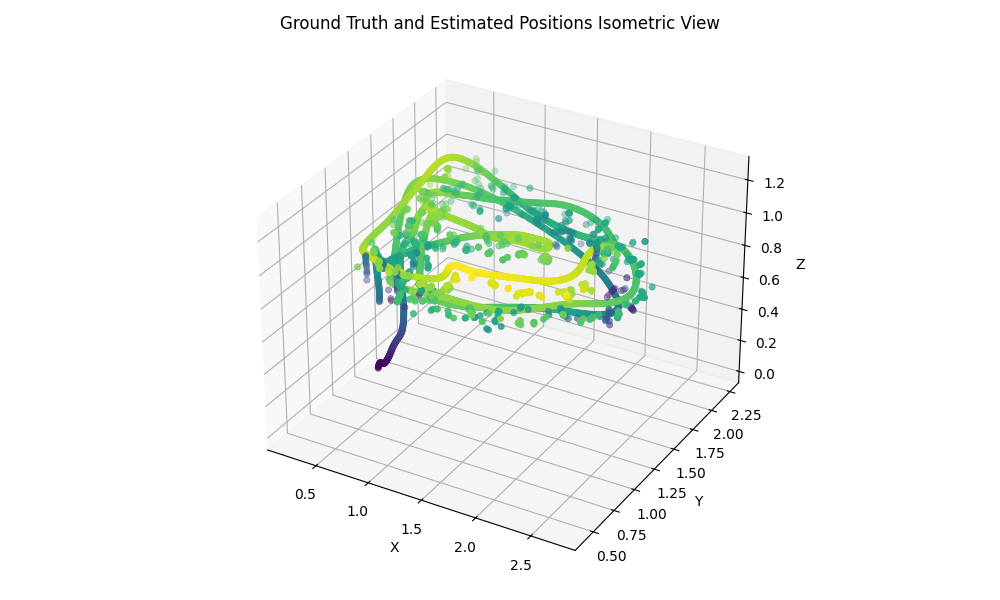
\includegraphics[width=0.8\textwidth]{./imgs/task1_2/studentdata0_isometric.png}
    \caption{Dataset 0 Isometric View}
\end{figure}

\begin{figure}[H]
    \centering
    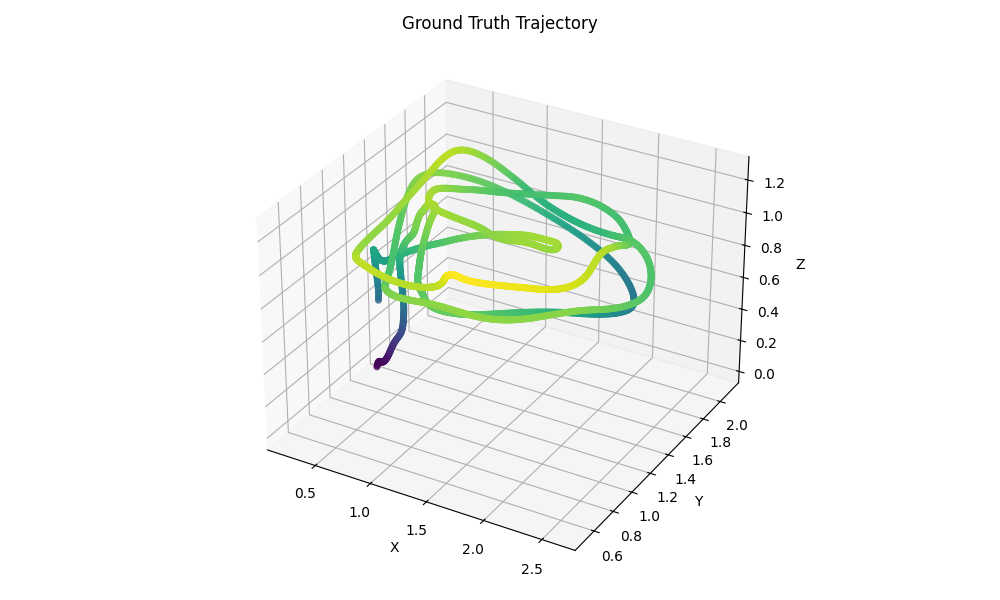
\includegraphics[width=0.8\textwidth]{./imgs/task1_2/studentdata0_ground_truth.png}
    \caption{Dataset 0 Ground Truth}
\end{figure}

\begin{figure}[H]
    \centering
    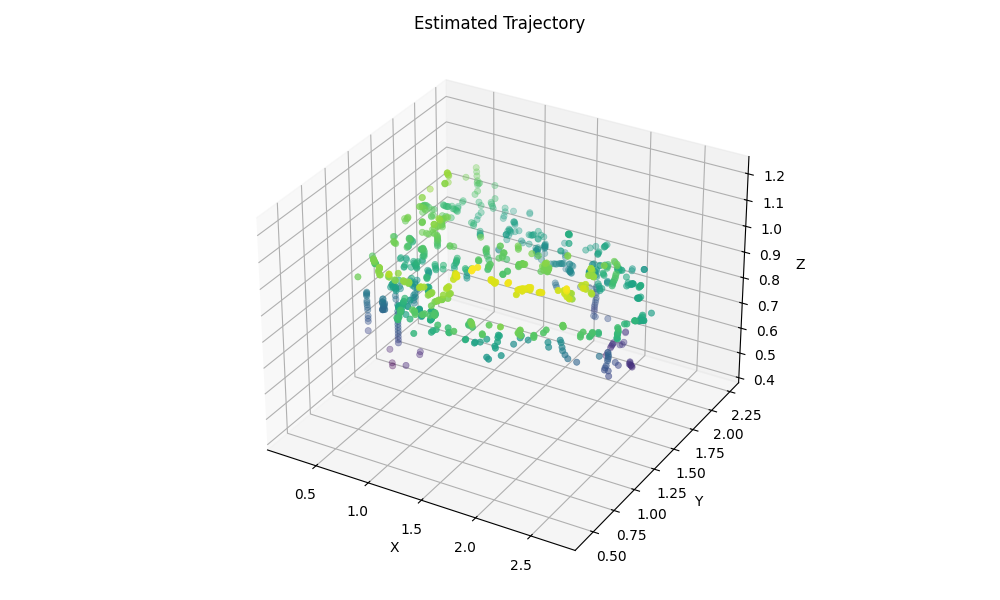
\includegraphics[width=0.8\textwidth]{./imgs/task1_2/studentdata0_estimated.png}
    \caption{Dataset 0 Estimated}
\end{figure}

\begin{figure}[H]
    \centering
    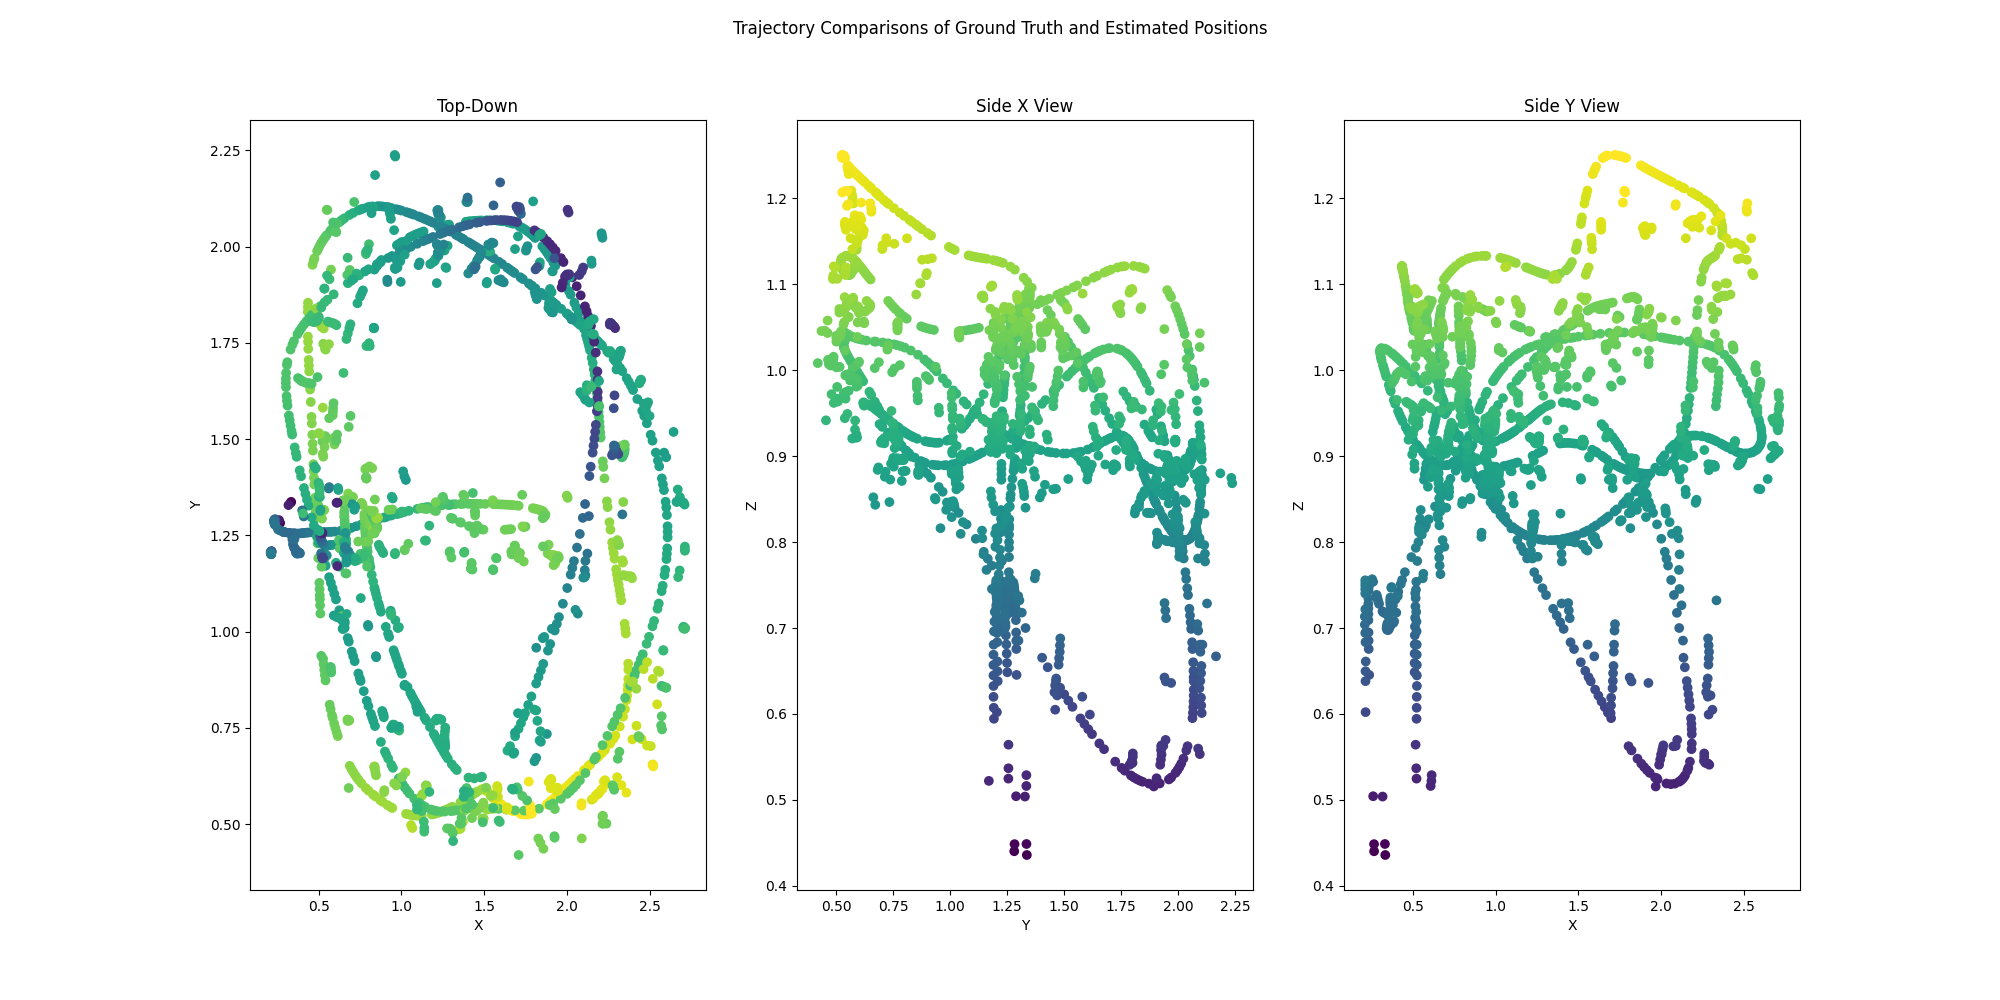
\includegraphics[width=0.8\textwidth]{./imgs/task1_2/studentdata0_trajectory_merged.png}
    \caption{Dataset 0 Trajectories}
\end{figure}

\begin{figure}[H]
    \centering
    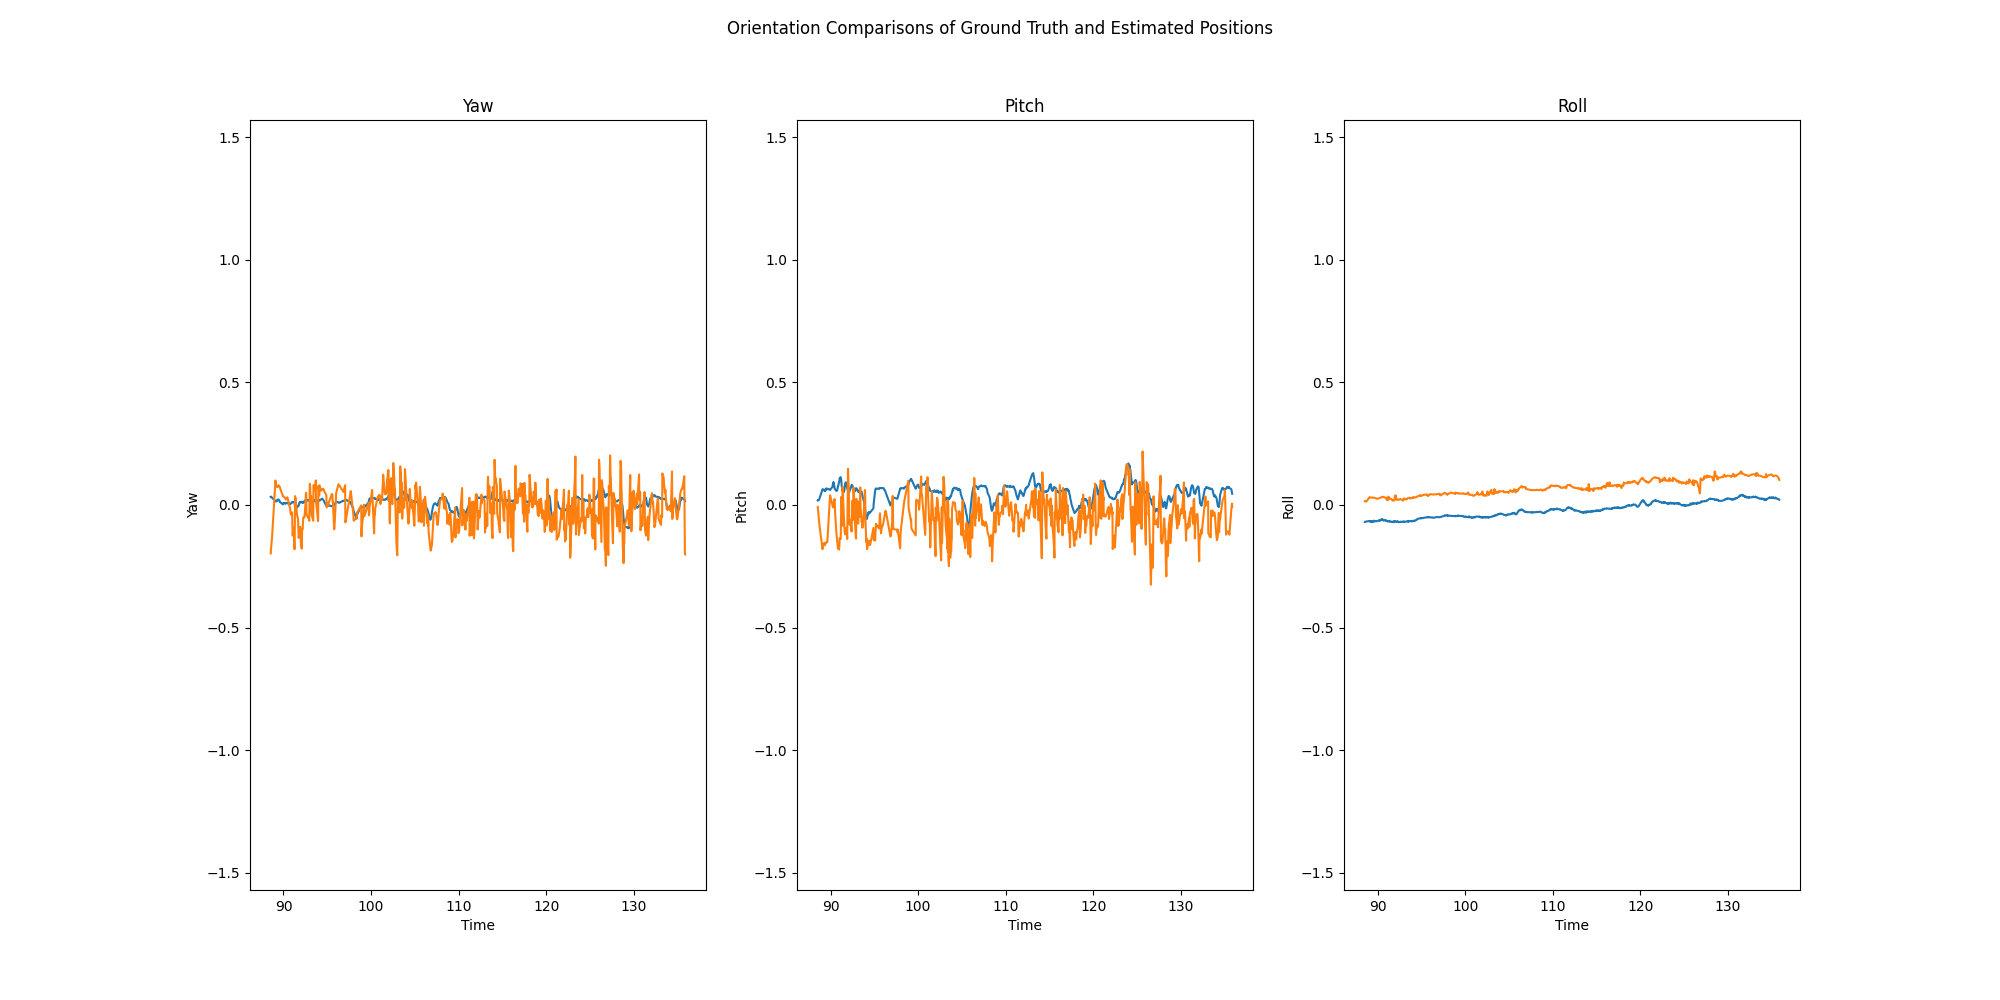
\includegraphics[width=0.8\textwidth]{./imgs/task1_2/studentdata0_orientation_merged.png}
    \caption{Dataset 0 Orientations}
\end{figure}

\subsection*{Dataset 1}

\begin{figure}[H]
    \centering
    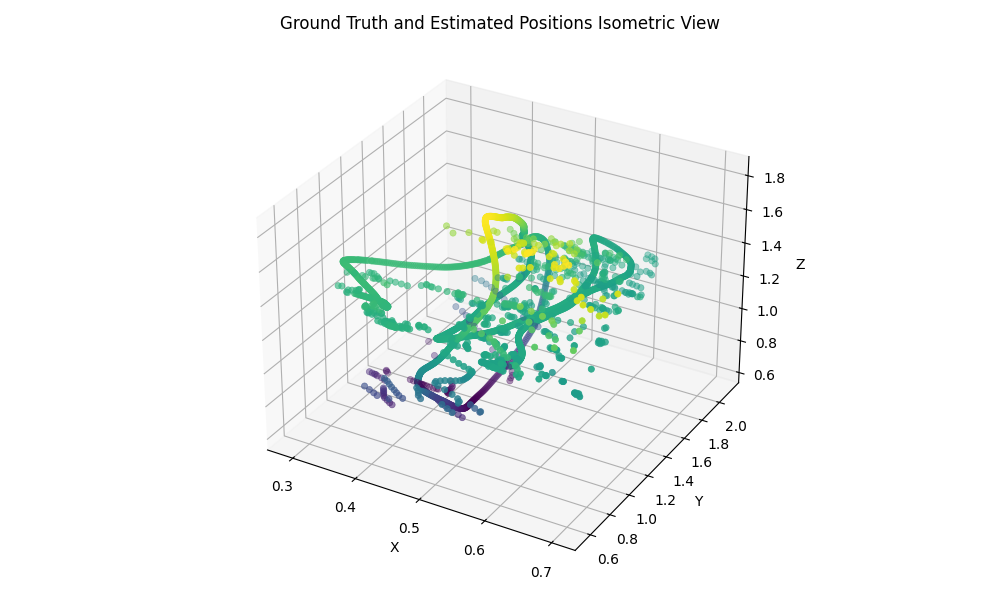
\includegraphics[width=0.8\textwidth]{./imgs/task1_2/studentdata1_isometric.png}
    \caption{Dataset 1 Isometric View}
\end{figure}

\begin{figure}[H]
    \centering
    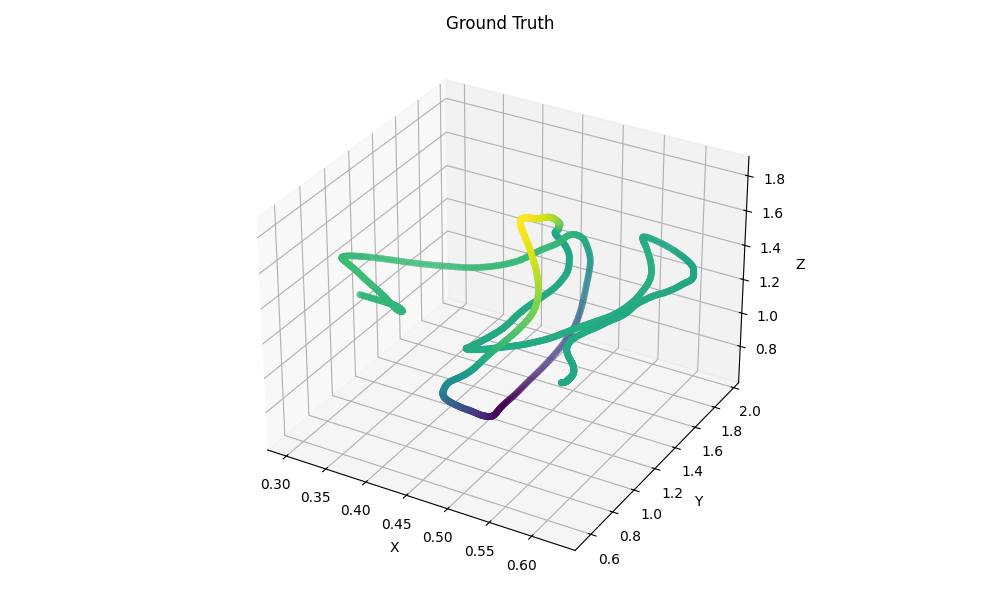
\includegraphics[width=0.8\textwidth]{./imgs/task1_2/studentdata1_ground_truth.png}
    \caption{Dataset 1 Ground Truth}
\end{figure}

\begin{figure}[H]
    \centering
    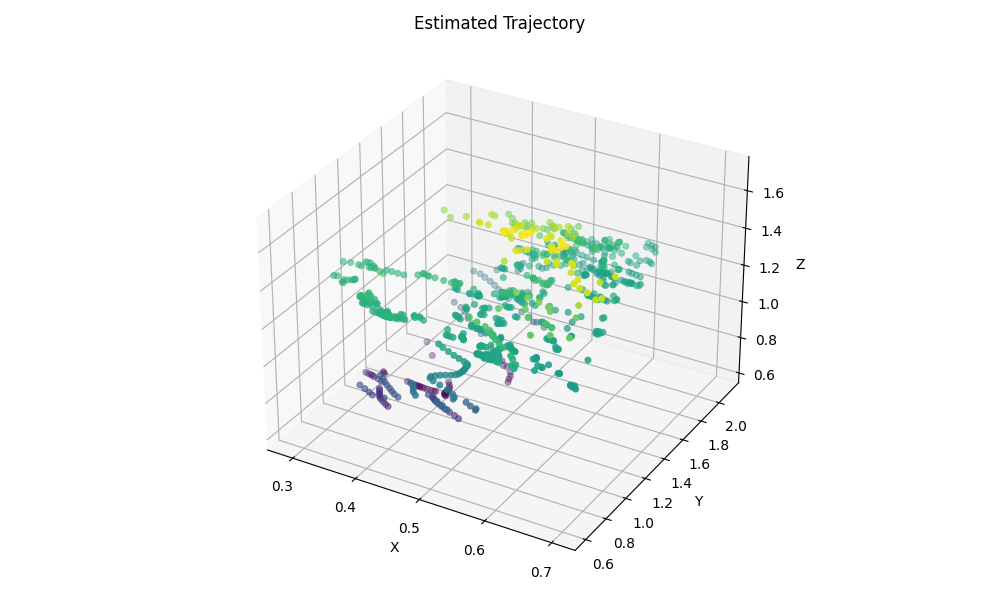
\includegraphics[width=0.8\textwidth]{./imgs/task1_2/studentdata1_estimated.png}
    \caption{Dataset 1 Estimated}
\end{figure}

\begin{figure}[H]
    \centering
    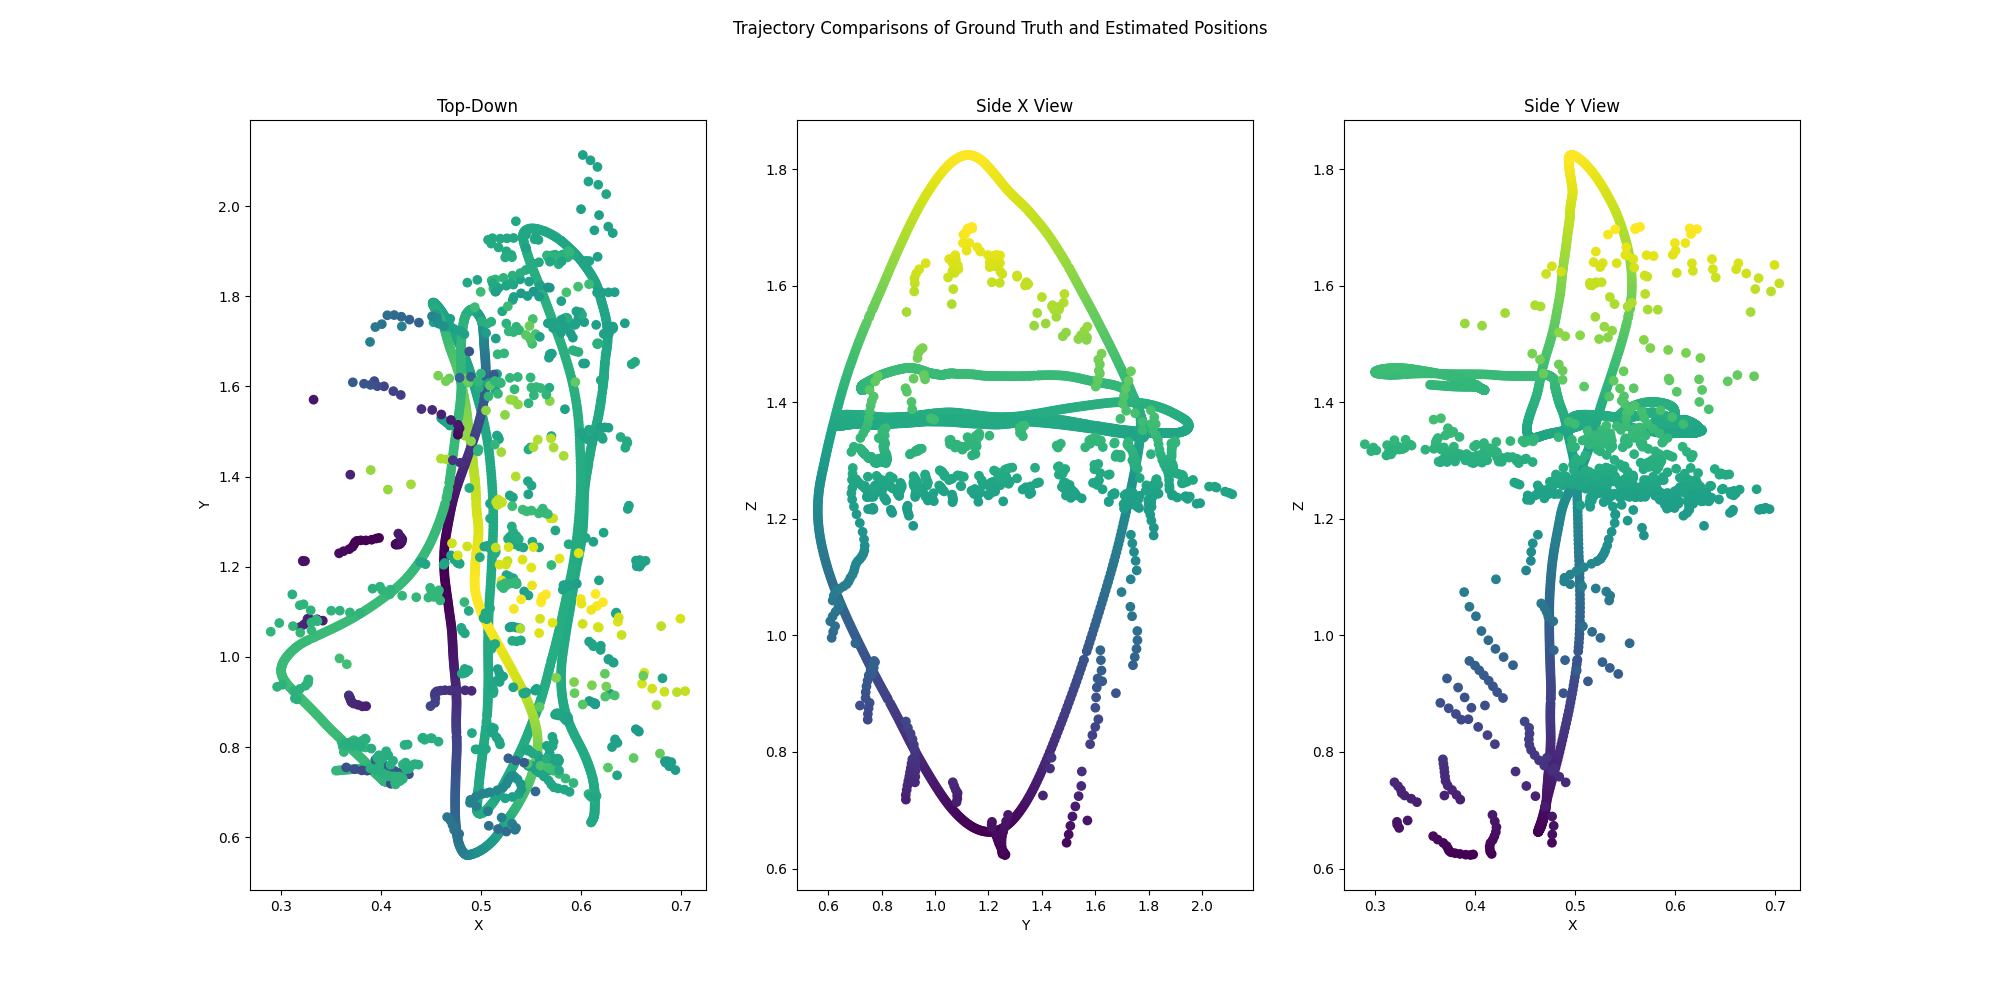
\includegraphics[width=0.8\textwidth]{./imgs/task1_2/studentdata1_trajectory_merged.png}
    \caption{Dataset 1 Trajectories}
\end{figure}

\begin{figure}[H]
    \centering
    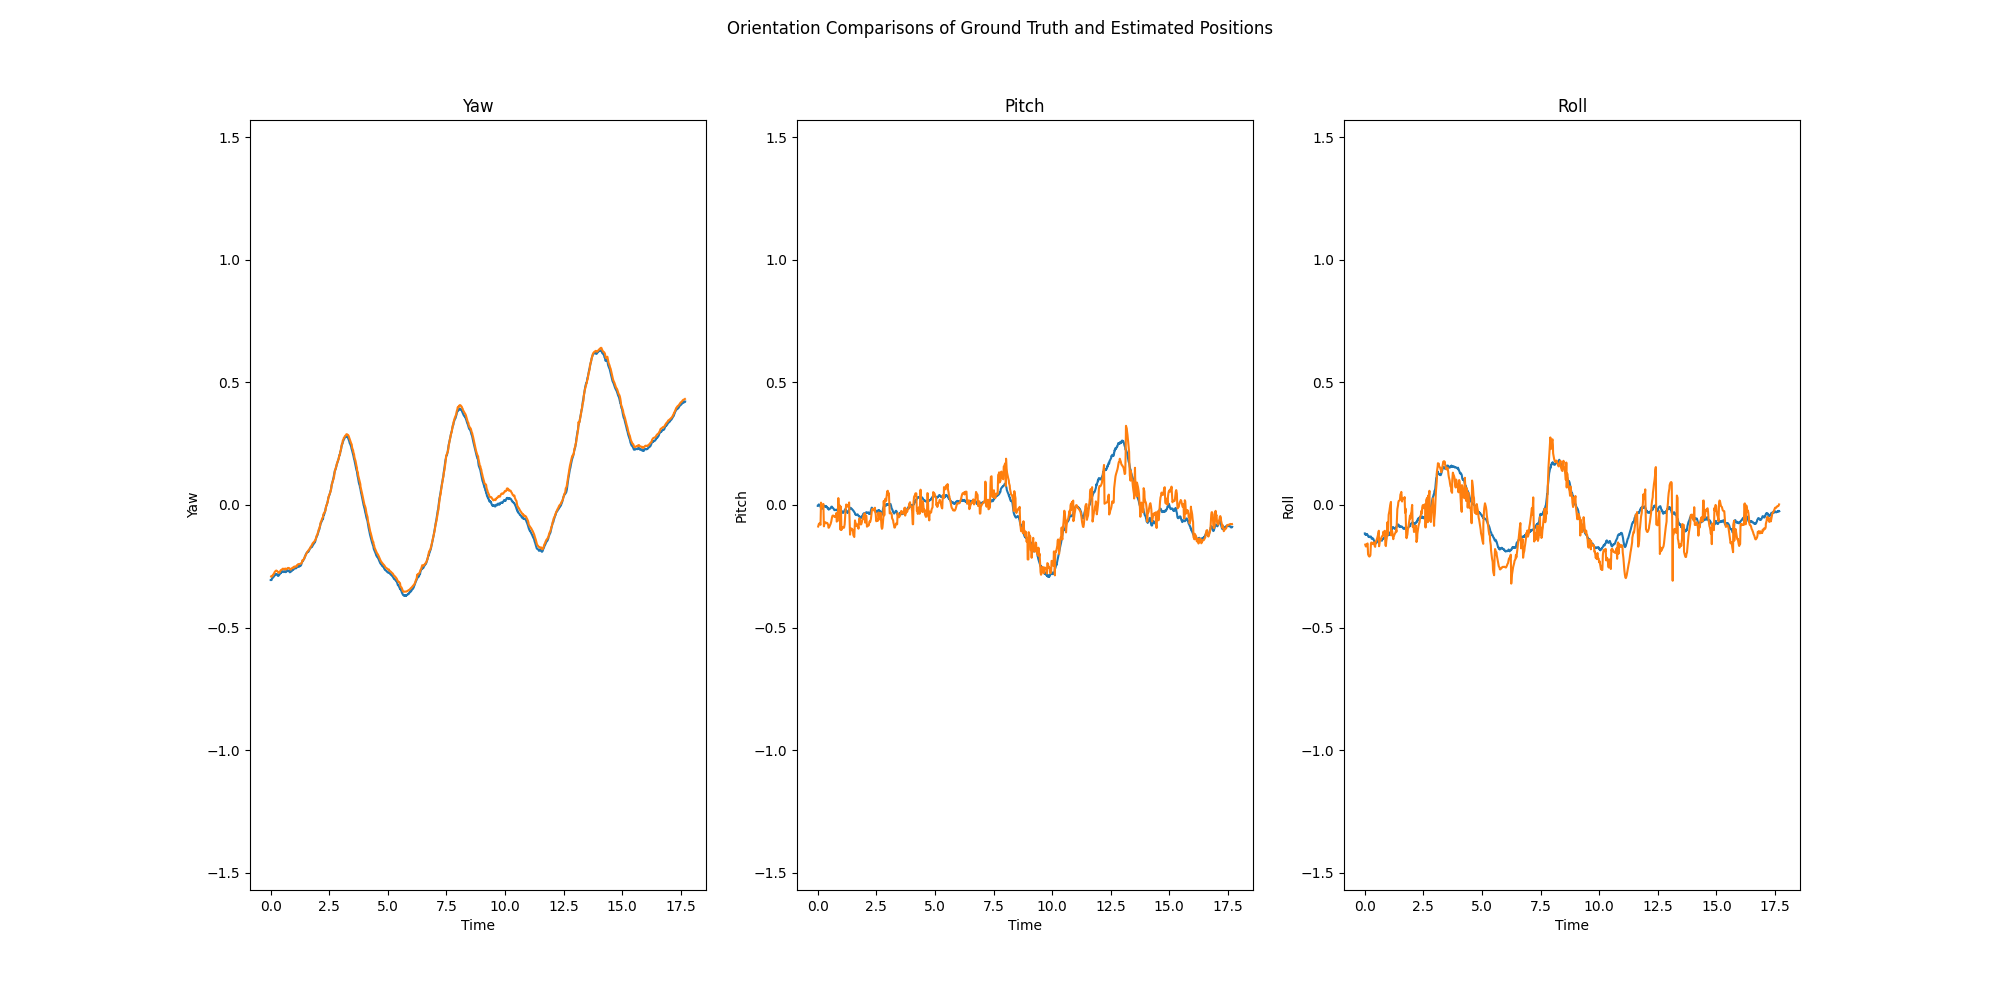
\includegraphics[width=0.8\textwidth]{./imgs/task1_2/studentdata1_orientation_merged.png}
    \caption{Dataset 1 Orientations}
\end{figure}

\subsection*{Dataset 2}

\begin{figure}[H]
    \centering
    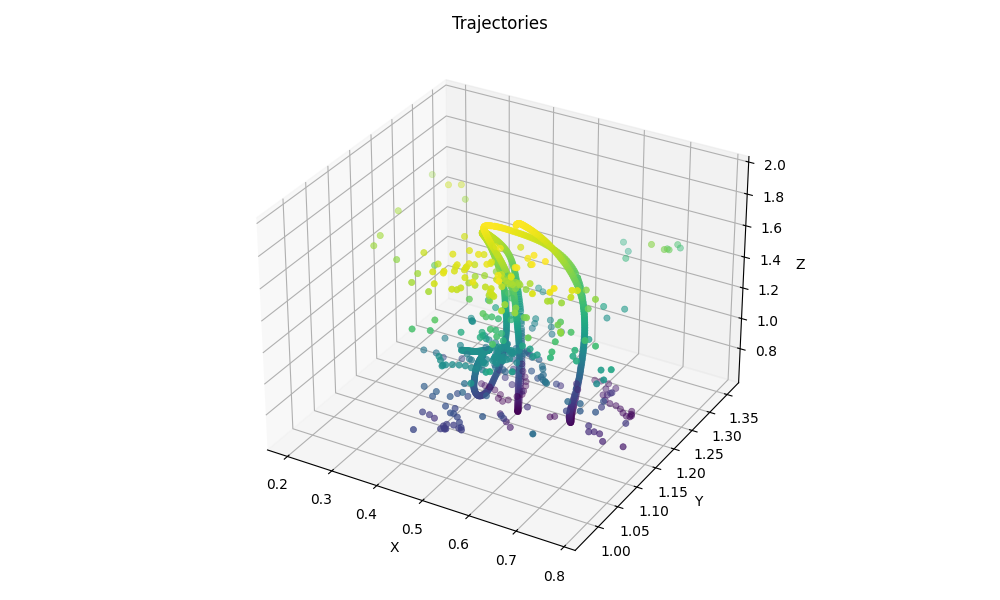
\includegraphics[width=0.8\textwidth]{./imgs/task1_2/studentdata2_isometric.png}
    \caption{Dataset 2 Isometric View}
\end{figure}

\begin{figure}[H]
    \centering
    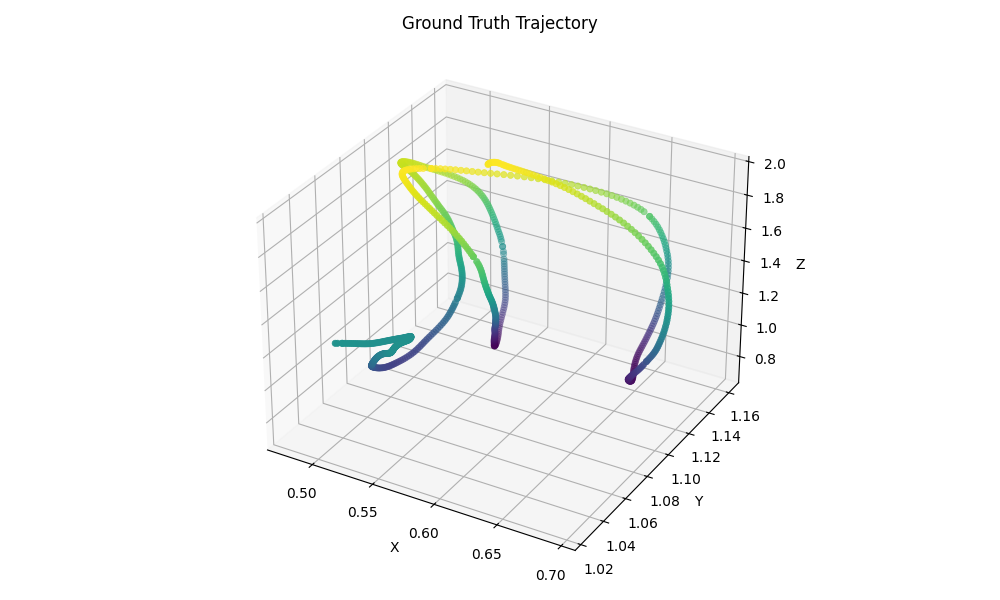
\includegraphics[width=0.8\textwidth]{./imgs/task1_2/studentdata2_ground_truth.png}
    \caption{Dataset 2 Ground Truth}
\end{figure}

\begin{figure}[H]
    \centering
    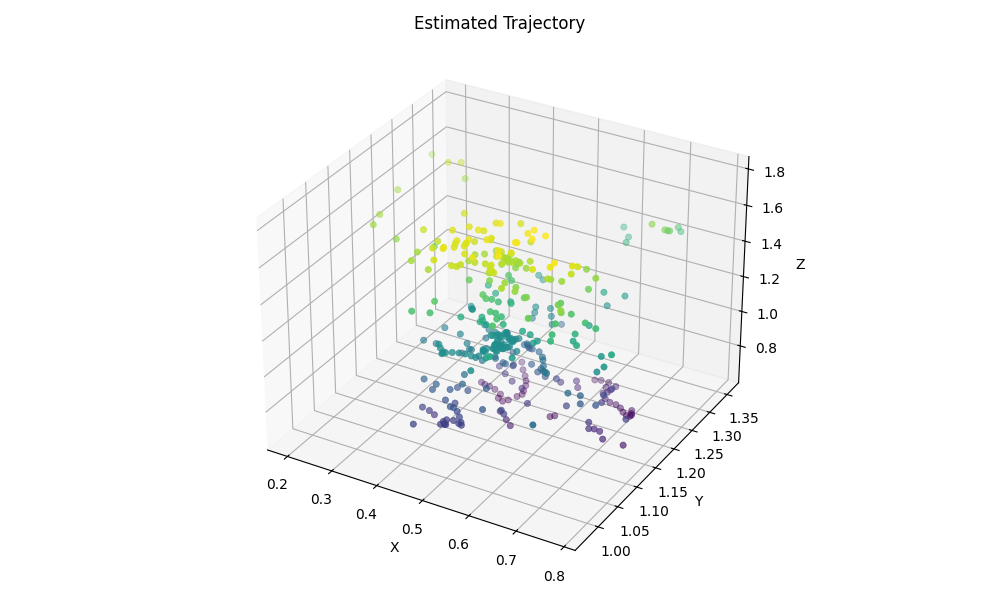
\includegraphics[width=0.8\textwidth]{./imgs/task1_2/studentdata2_estimated.png}
    \caption{Dataset 2 Estimated}
\end{figure}

\begin{figure}[H]
    \centering
    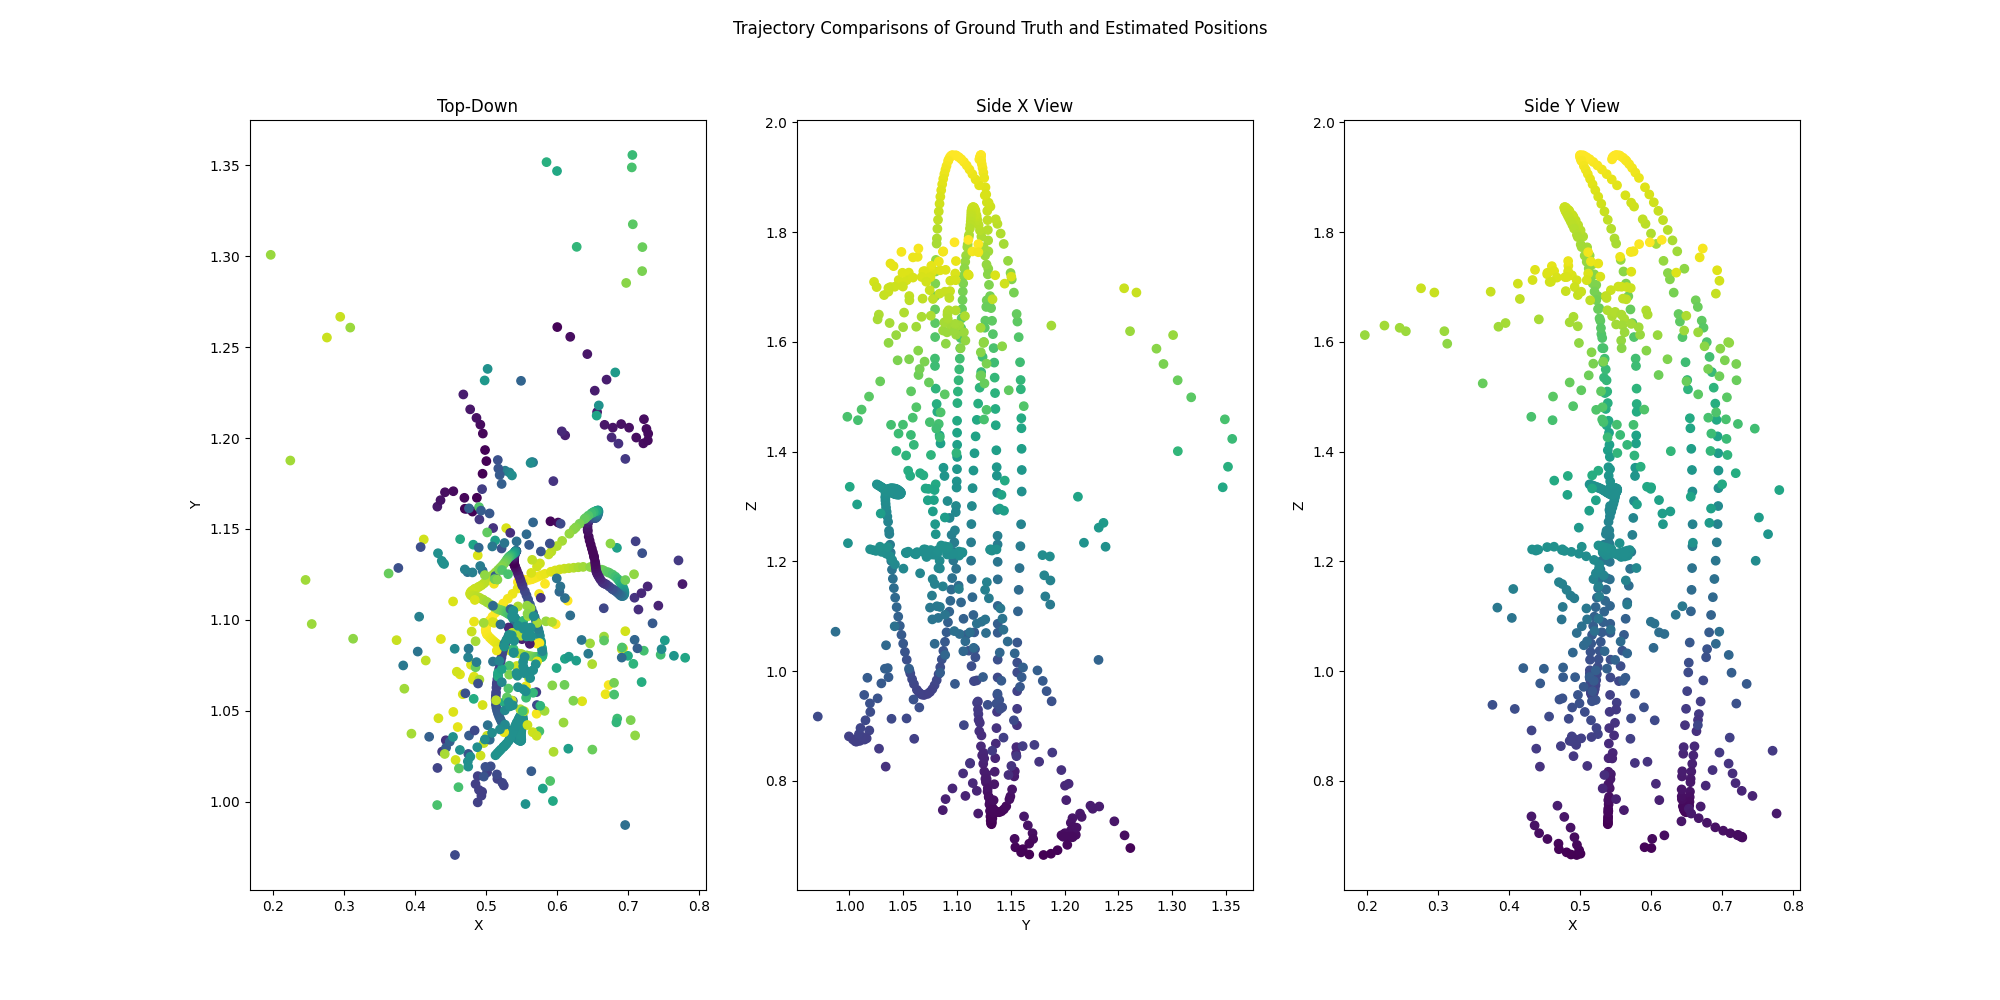
\includegraphics[width=0.8\textwidth]{./imgs/task1_2/studentdata2_trajectory_merged.png}
    \caption{Dataset 2 Trajectories}
\end{figure}

\begin{figure}[H]
    \centering
    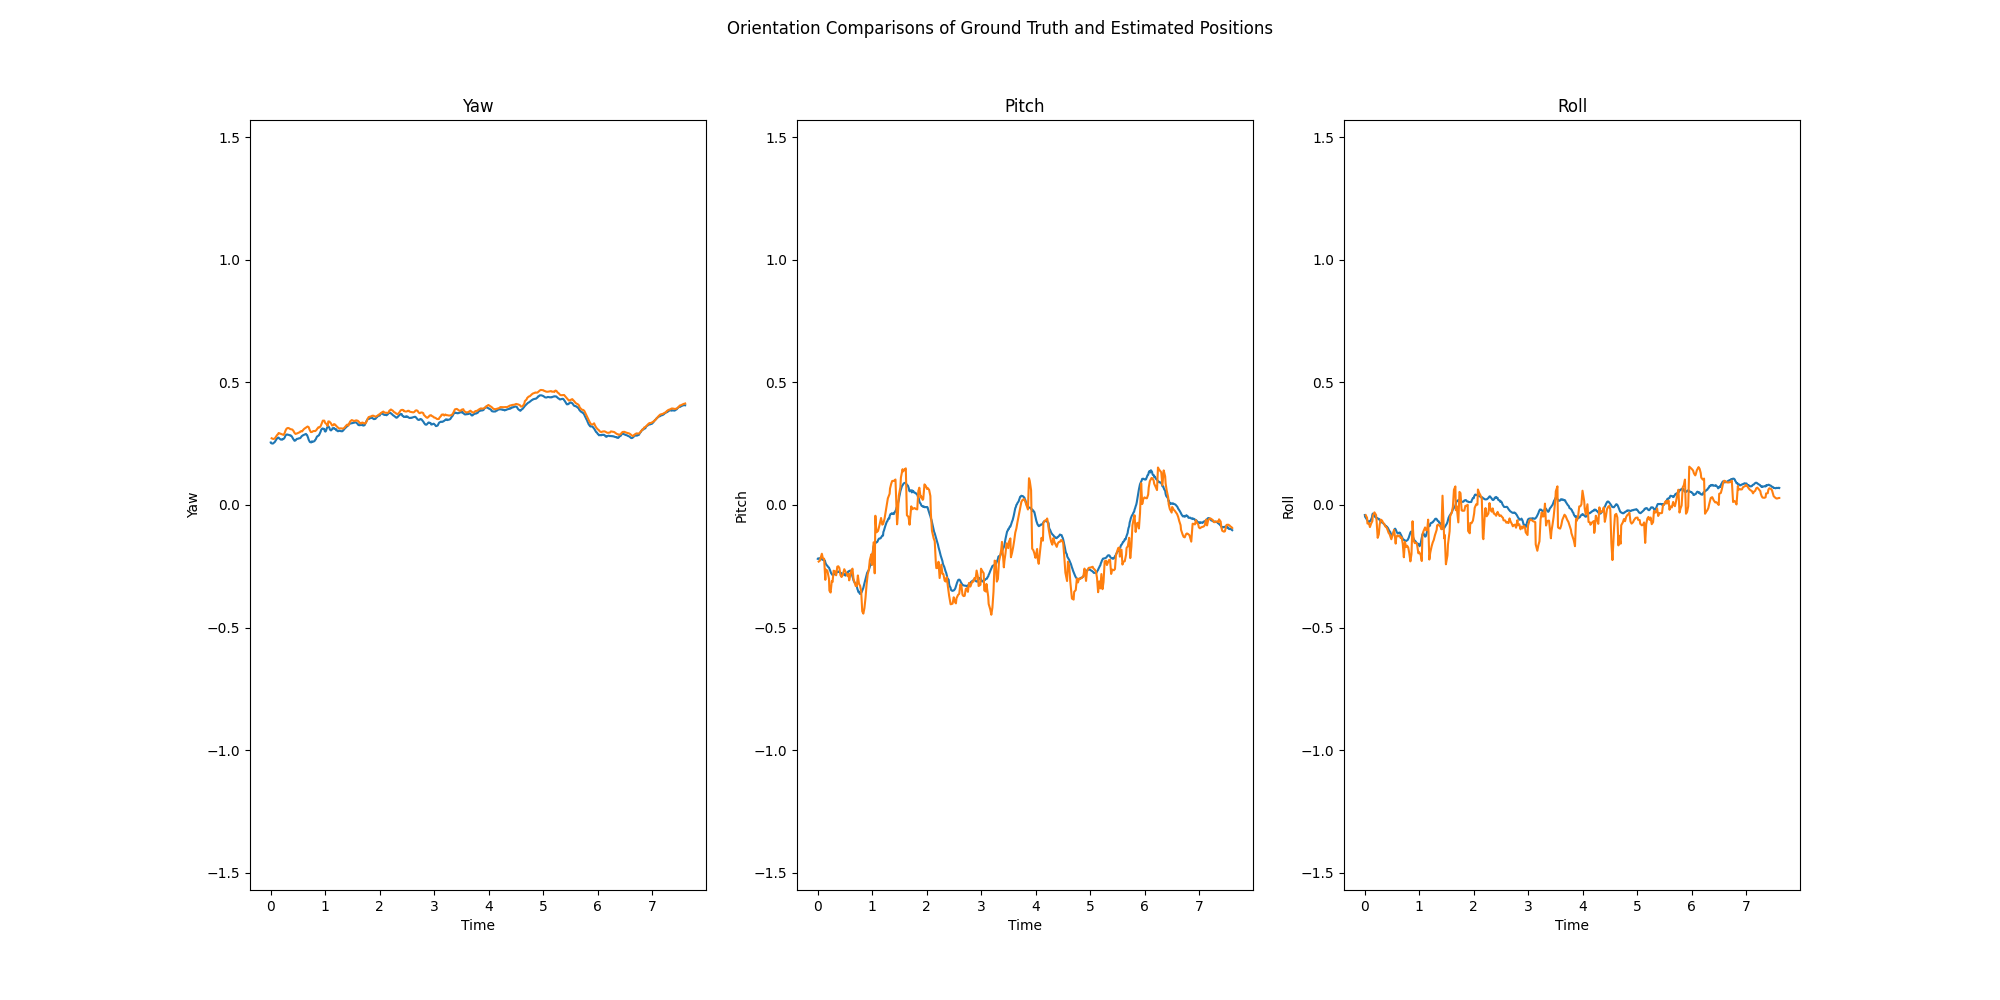
\includegraphics[width=0.8\textwidth]{./imgs/task1_2/studentdata2_orientation_merged.png}
    \caption{Dataset 2 Orientations}
\end{figure}

\subsection*{Dataset 3}

\begin{figure}[H]
    \centering
    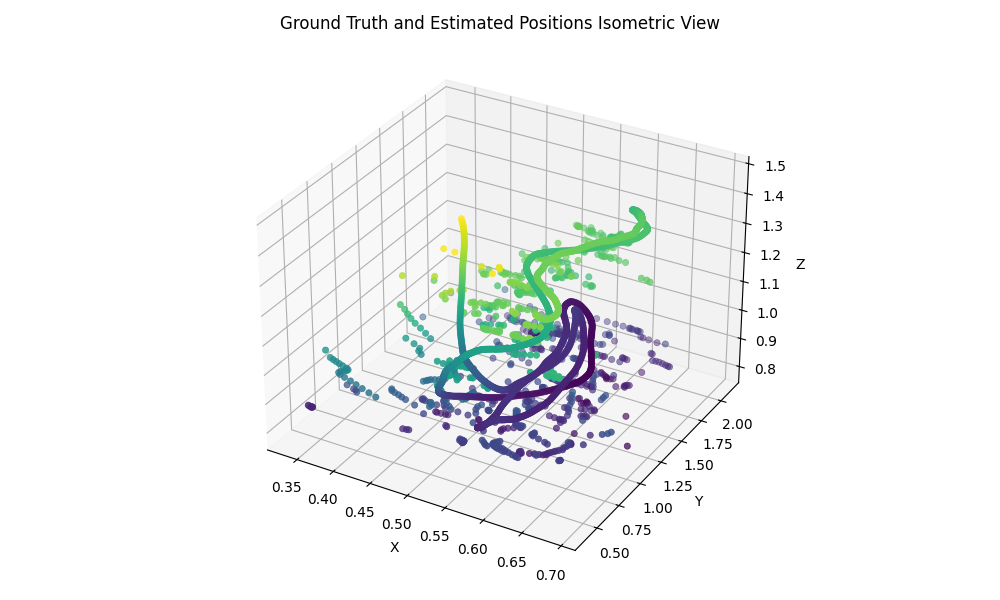
\includegraphics[width=0.8\textwidth]{./imgs/task1_2/studentdata3_isometric.png}
    \caption{Dataset 3 Isometric View}
\end{figure}

\begin{figure}[H]
    \centering
    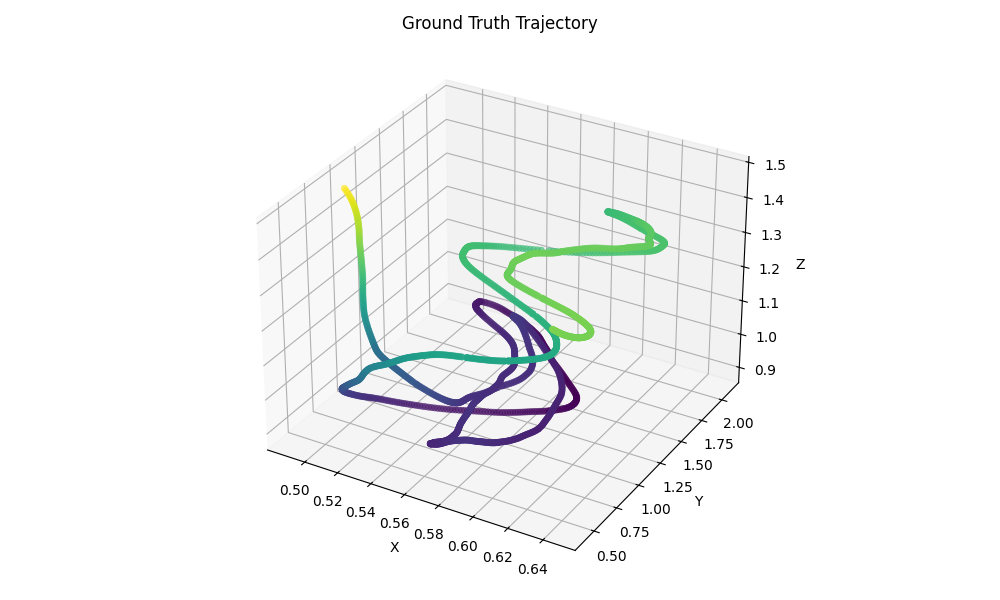
\includegraphics[width=0.8\textwidth]{./imgs/task1_2/studentdata3_ground_truth.png}
    \caption{Dataset 3 Ground Truth}
\end{figure}

\begin{figure}[H]
    \centering
    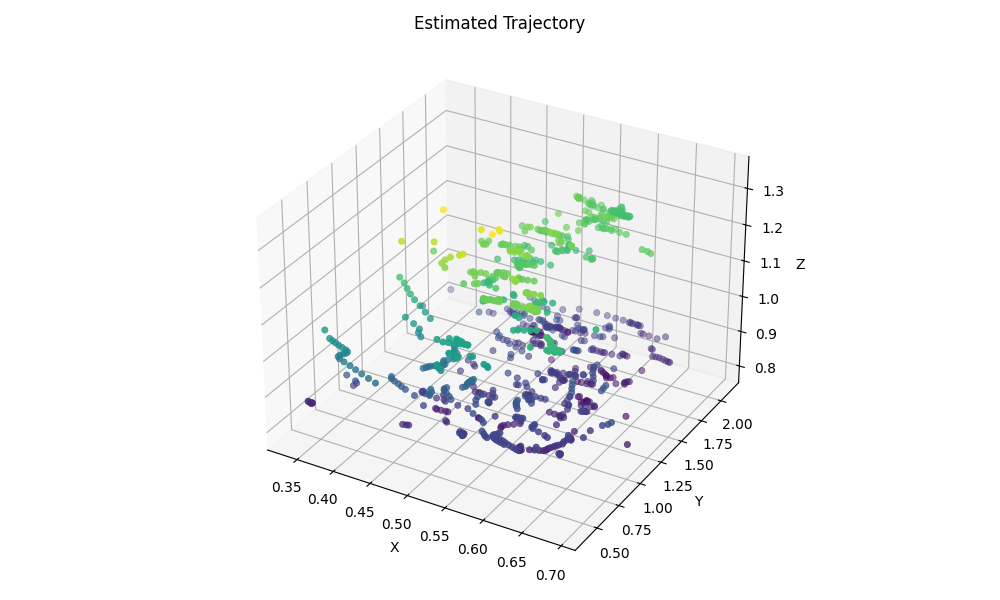
\includegraphics[width=0.8\textwidth]{./imgs/task1_2/studentdata3_estimated.png}
    \caption{Dataset 3 Estimated}
\end{figure}

\begin{figure}[H]
    \centering
    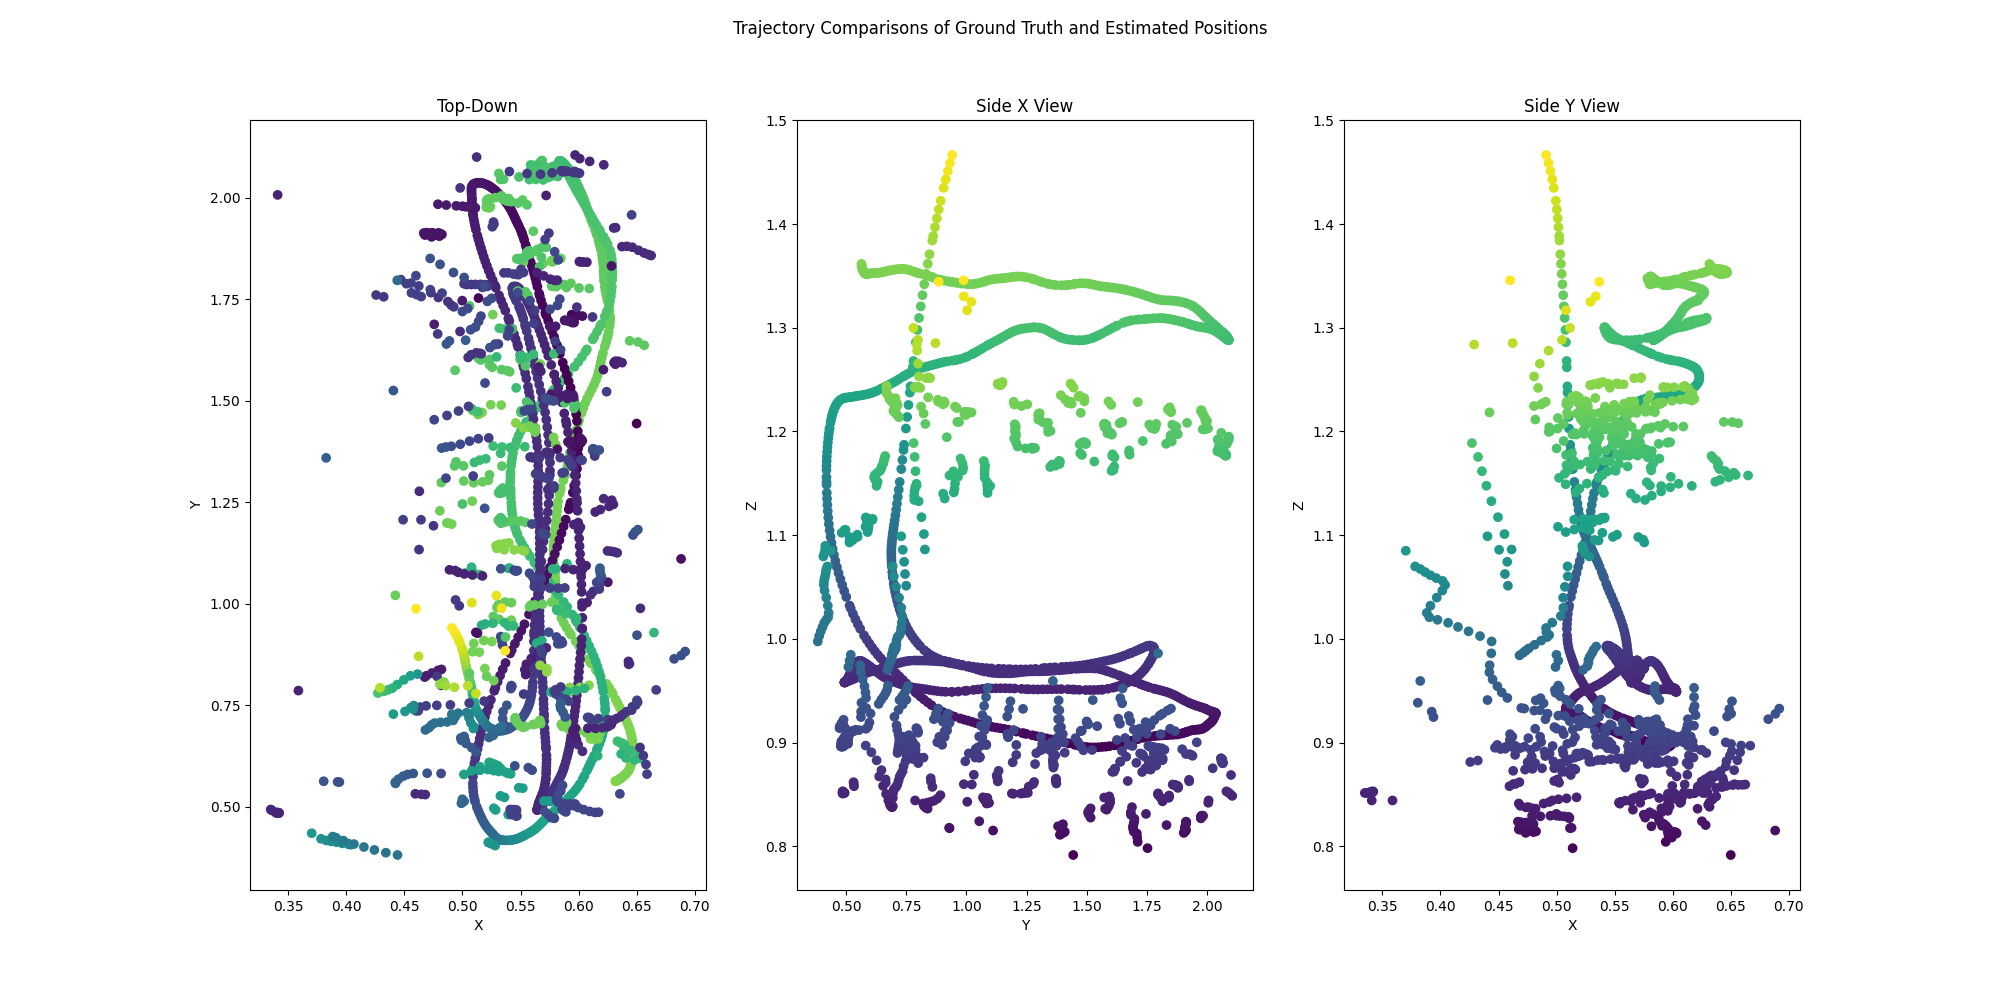
\includegraphics[width=0.8\textwidth]{./imgs/task1_2/studentdata3_trajectory_merged.png}
    \caption{Dataset 3 Trajectories}
\end{figure}

\begin{figure}[H]
    \centering
    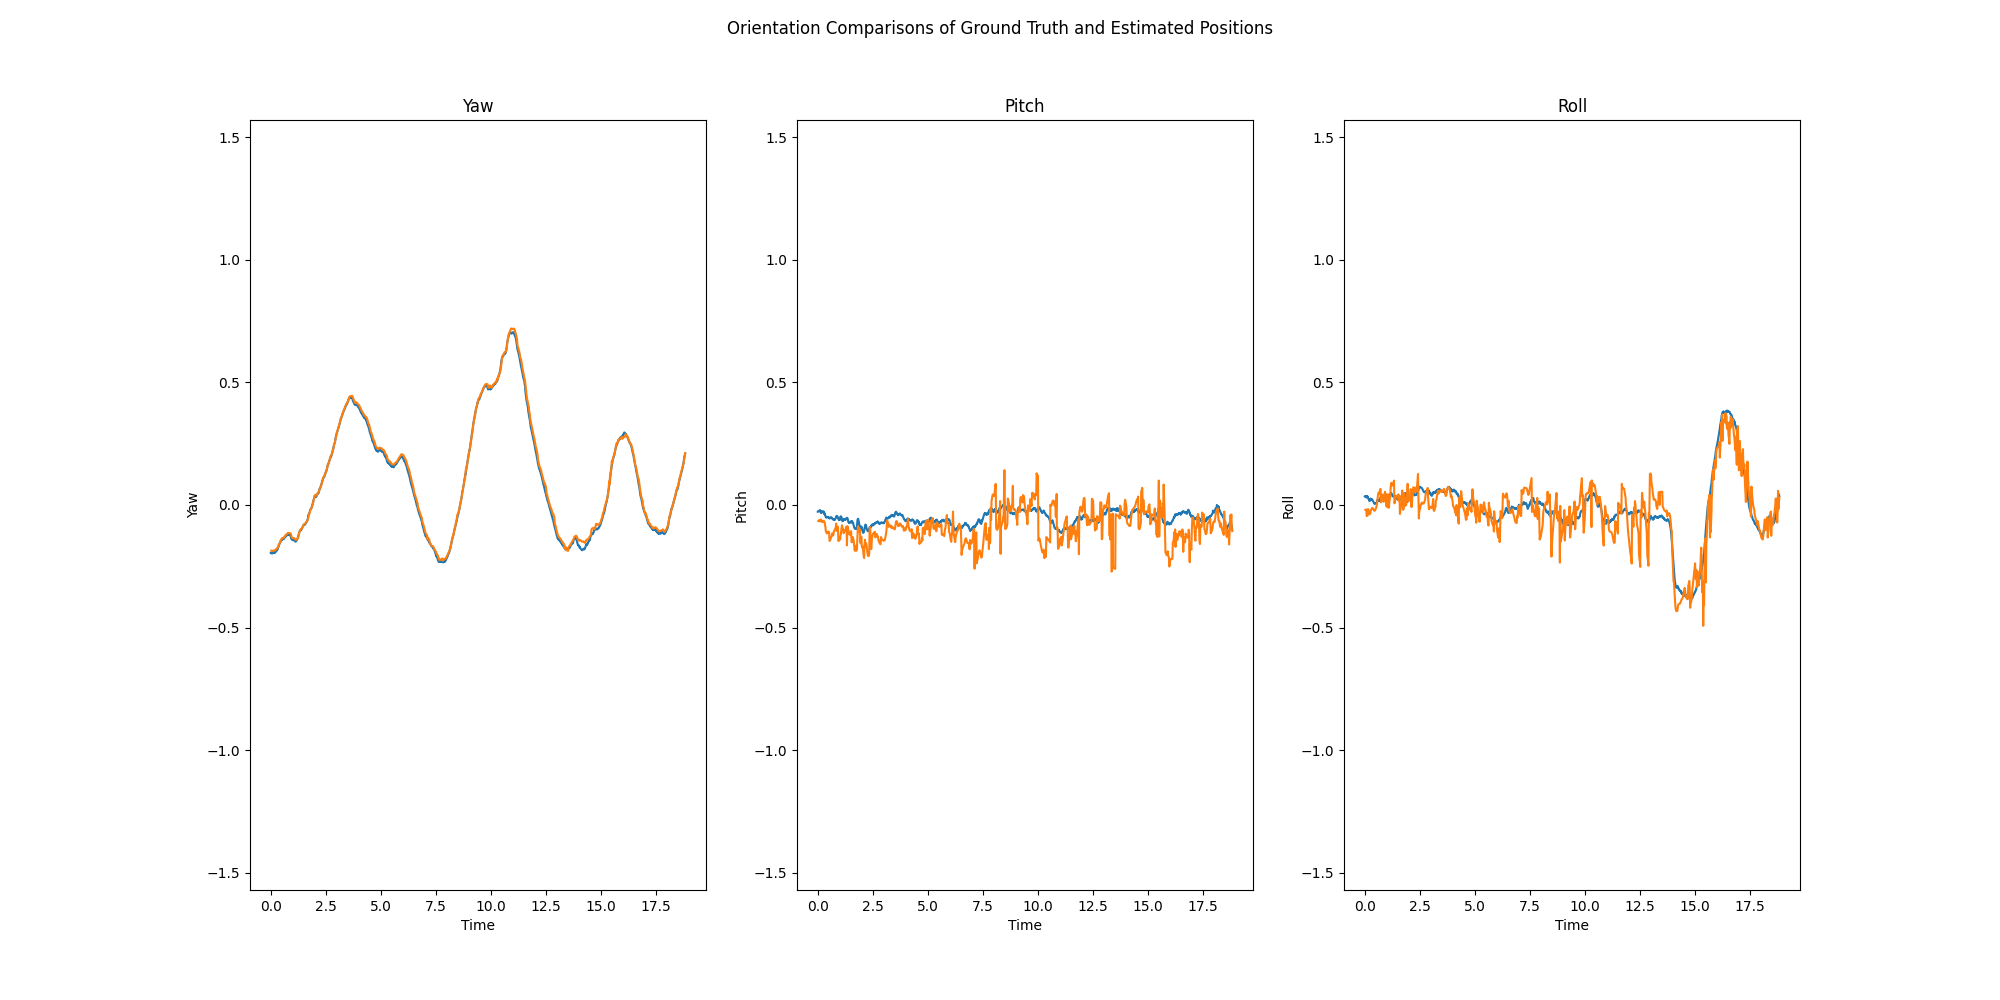
\includegraphics[width=0.8\textwidth]{./imgs/task1_2/studentdata3_orientation_merged.png}
    \caption{Dataset 3 Orientations}
\end{figure}

\subsection*{Dataset 4}

\begin{figure}[H]
    \centering
    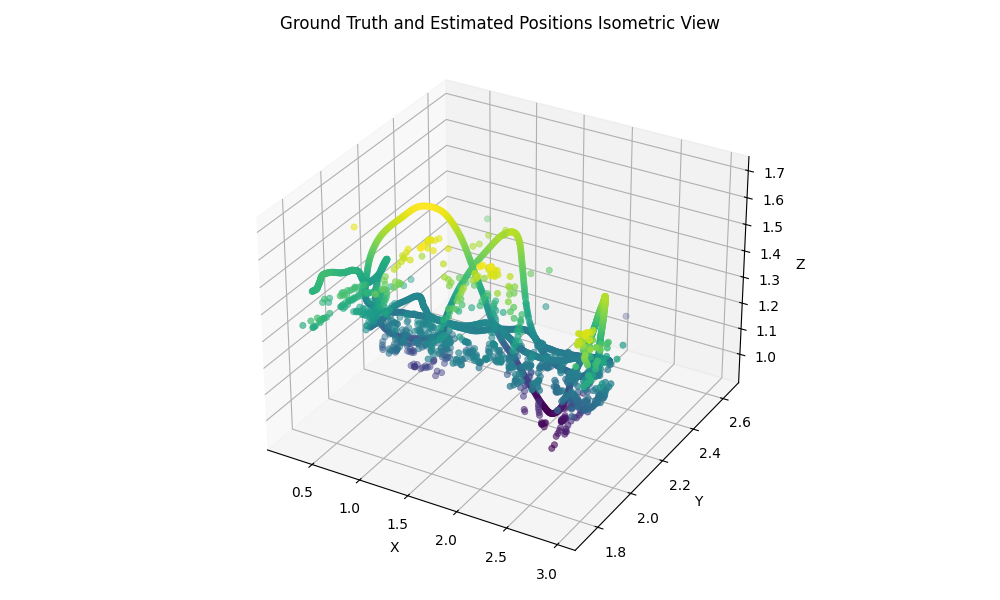
\includegraphics[width=0.8\textwidth]{./imgs/task1_2/studentdata4_isometric.png}
    \caption{Dataset 4 Isometric View}
\end{figure}

\begin{figure}[H]
    \centering
    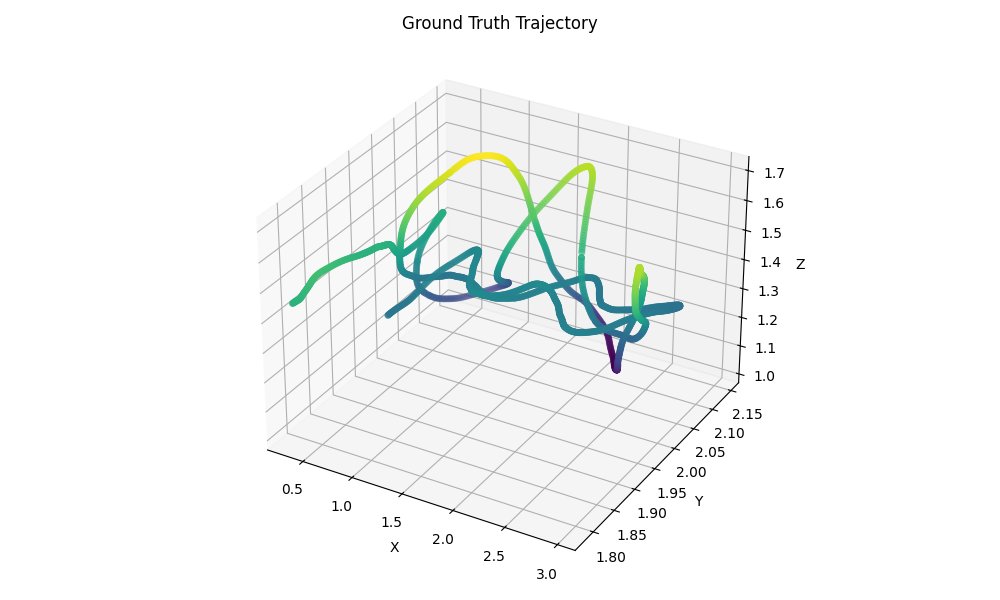
\includegraphics[width=0.8\textwidth]{./imgs/task1_2/studentdata4_ground_truth.png}
    \caption{Dataset 4 Ground Truth}
\end{figure}

\begin{figure}[H]
    \centering
    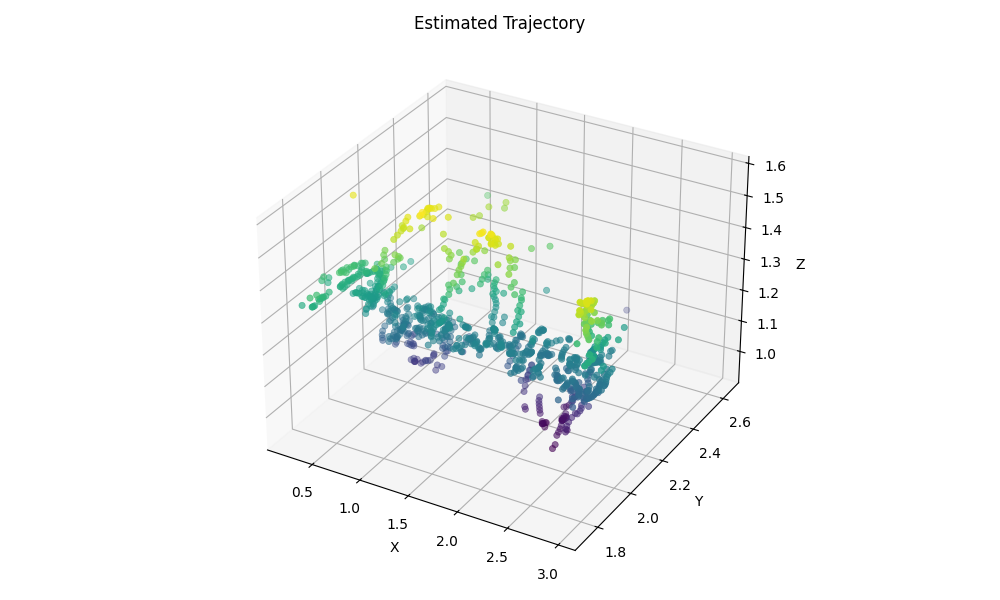
\includegraphics[width=0.8\textwidth]{./imgs/task1_2/studentdata4_estimated.png}
    \caption{Dataset 4 Estimated}
\end{figure}

\begin{figure}[H]
    \centering
    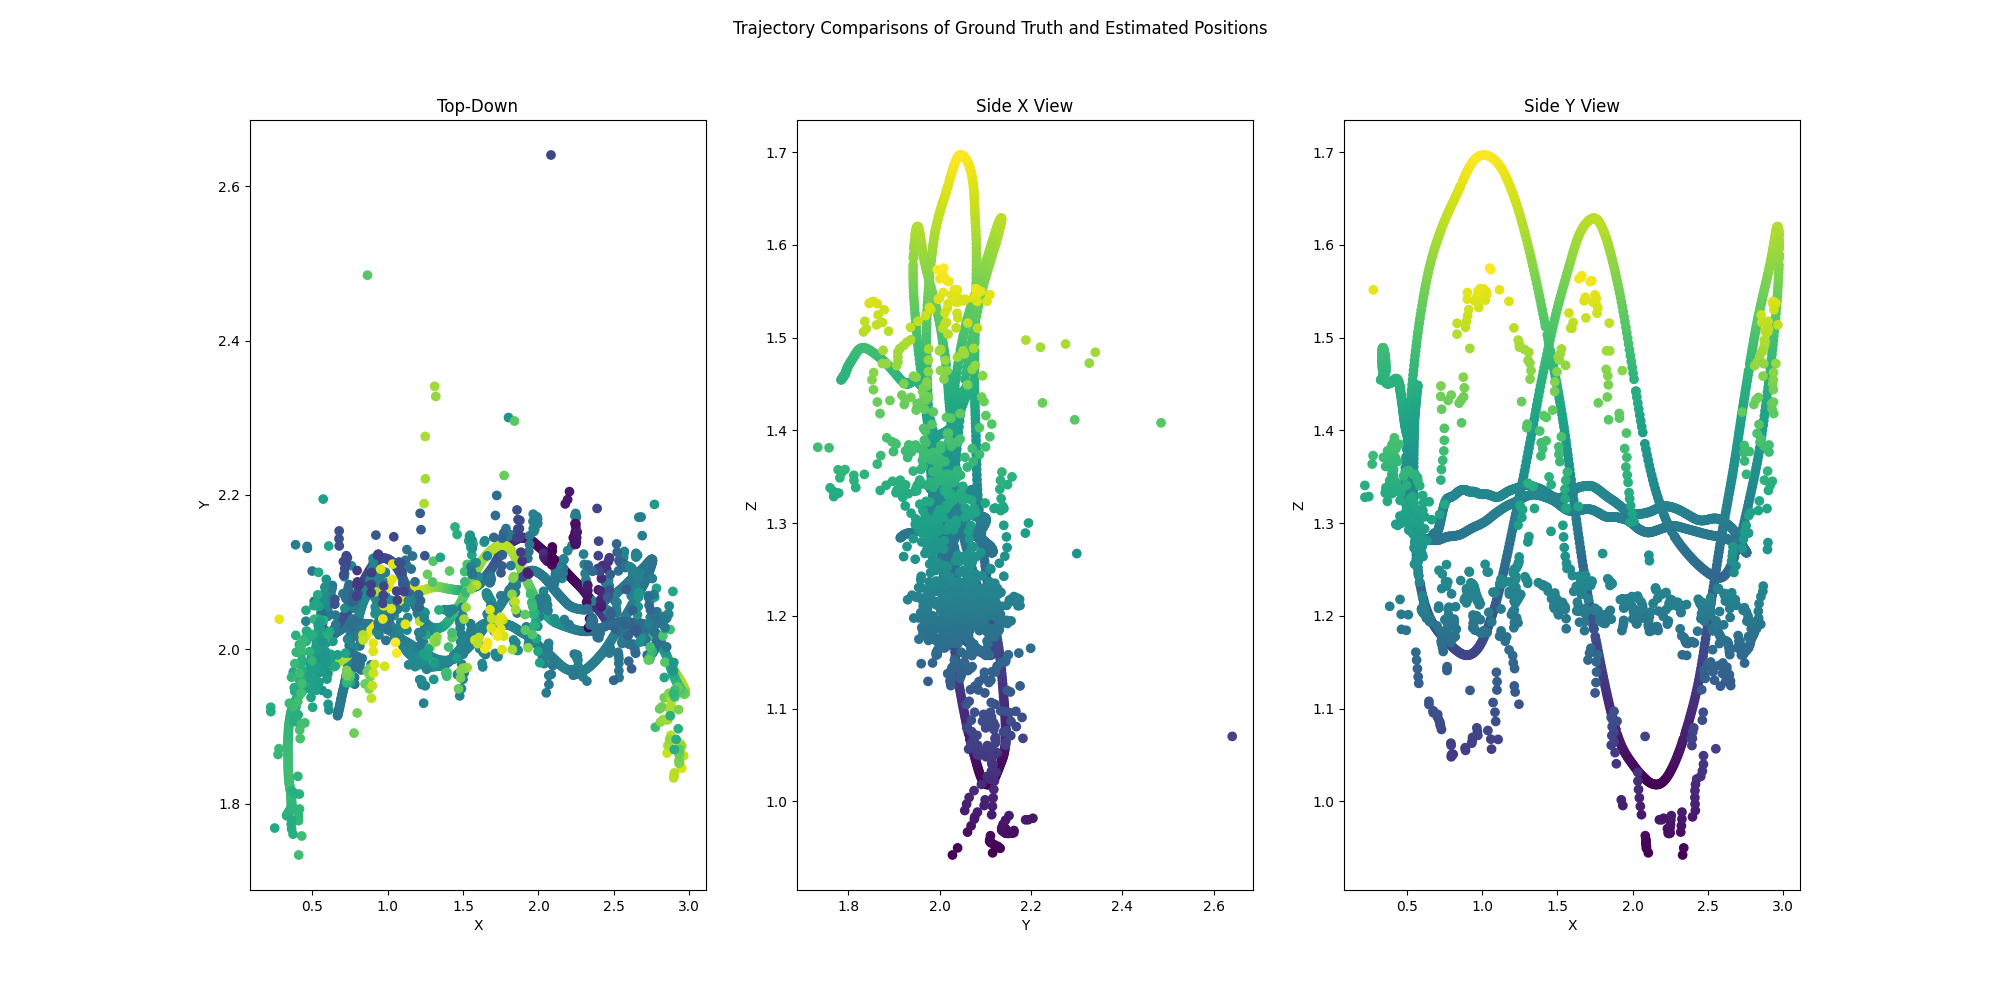
\includegraphics[width=0.8\textwidth]{./imgs/task1_2/studentdata4_trajectory_merged.png}
    \caption{Dataset 4 Trajectories}
\end{figure}

\begin{figure}[H]
    \centering
    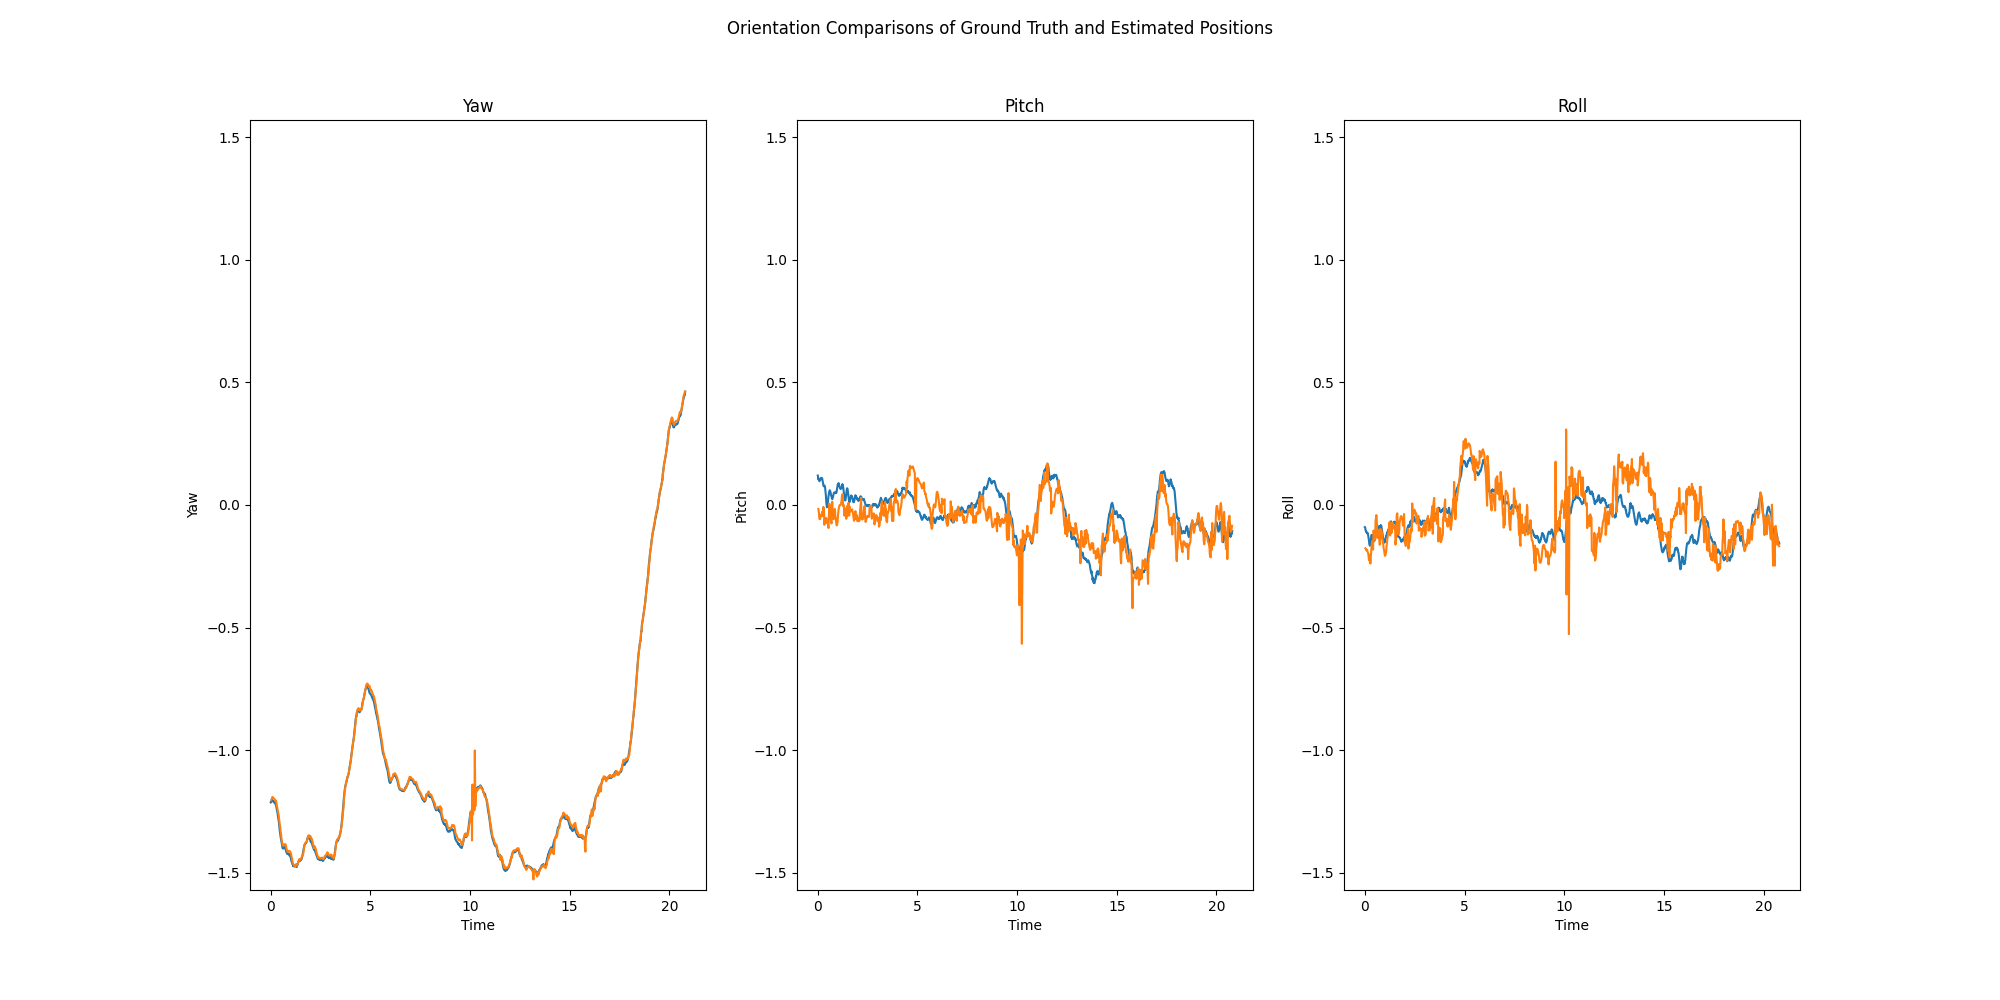
\includegraphics[width=0.8\textwidth]{./imgs/task1_2/studentdata4_orientation_merged.png}
    \caption{Dataset 4 Orientations}
\end{figure}

\subsection*{Dataset 5}

\begin{figure}[H]
    \centering
    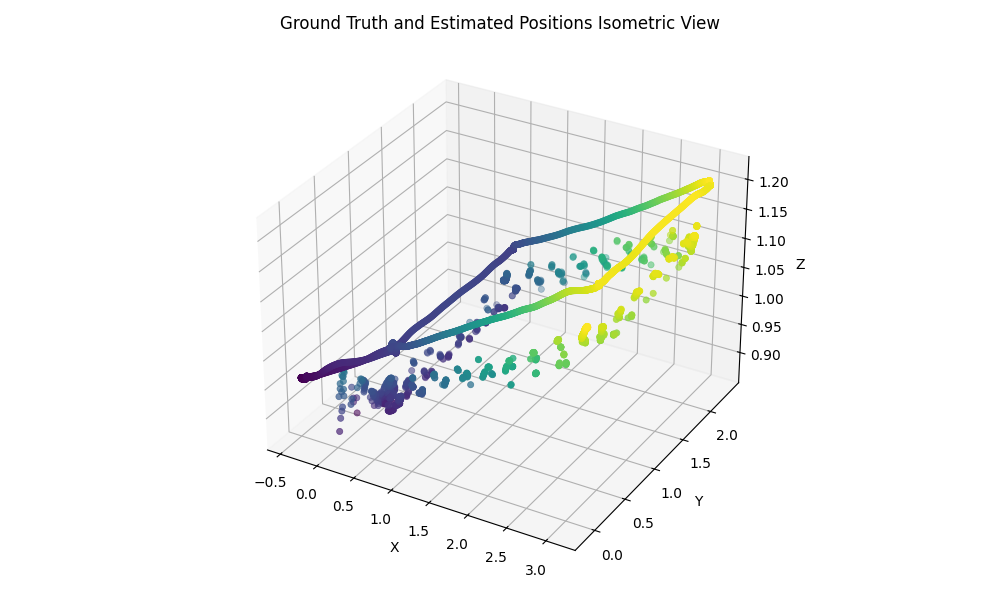
\includegraphics[width=0.8\textwidth]{./imgs/task1_2/studentdata5_isometric.png}
    \caption{Dataset 5 Isometric View}
\end{figure}

\begin{figure}[H]
    \centering
    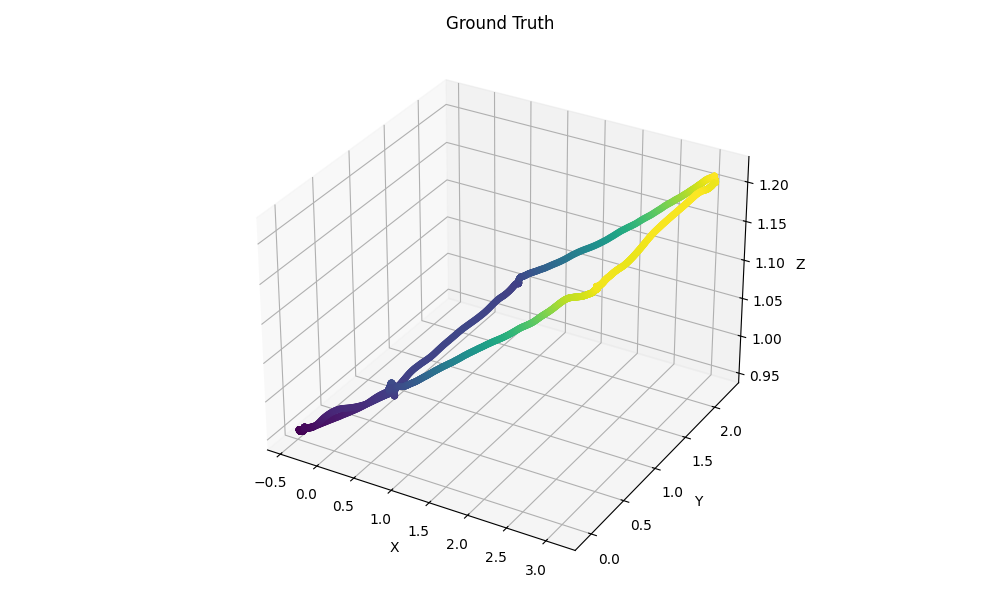
\includegraphics[width=0.8\textwidth]{./imgs/task1_2/studentdata5_ground_truth.png}
    \caption{Dataset 5 Ground Truth}
\end{figure}

\begin{figure}[H]
    \centering
    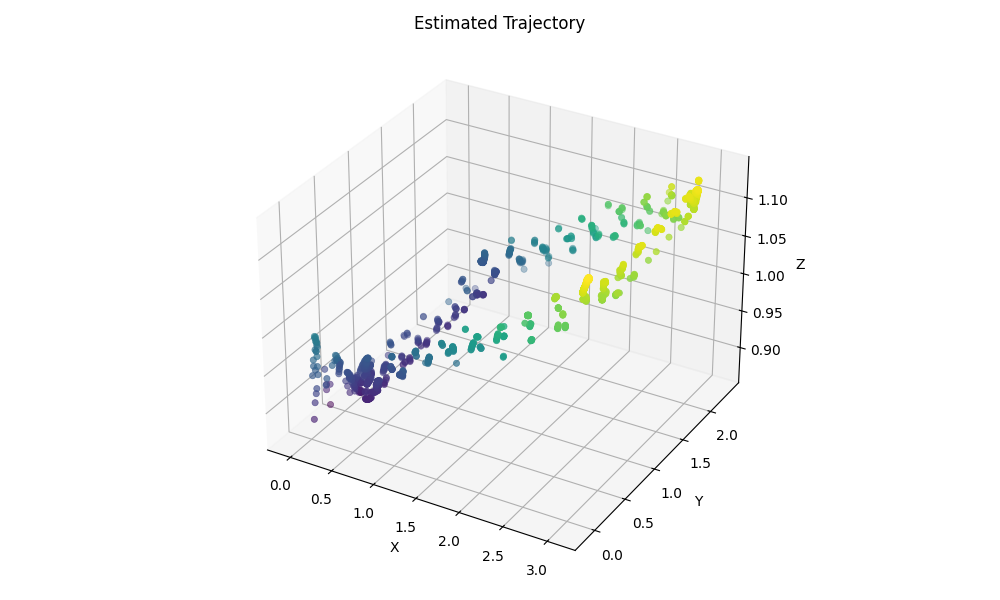
\includegraphics[width=0.8\textwidth]{./imgs/task1_2/studentdata5_estimated.png}
    \caption{Dataset 5 Estimated}
\end{figure}

\begin{figure}[H]
    \centering
    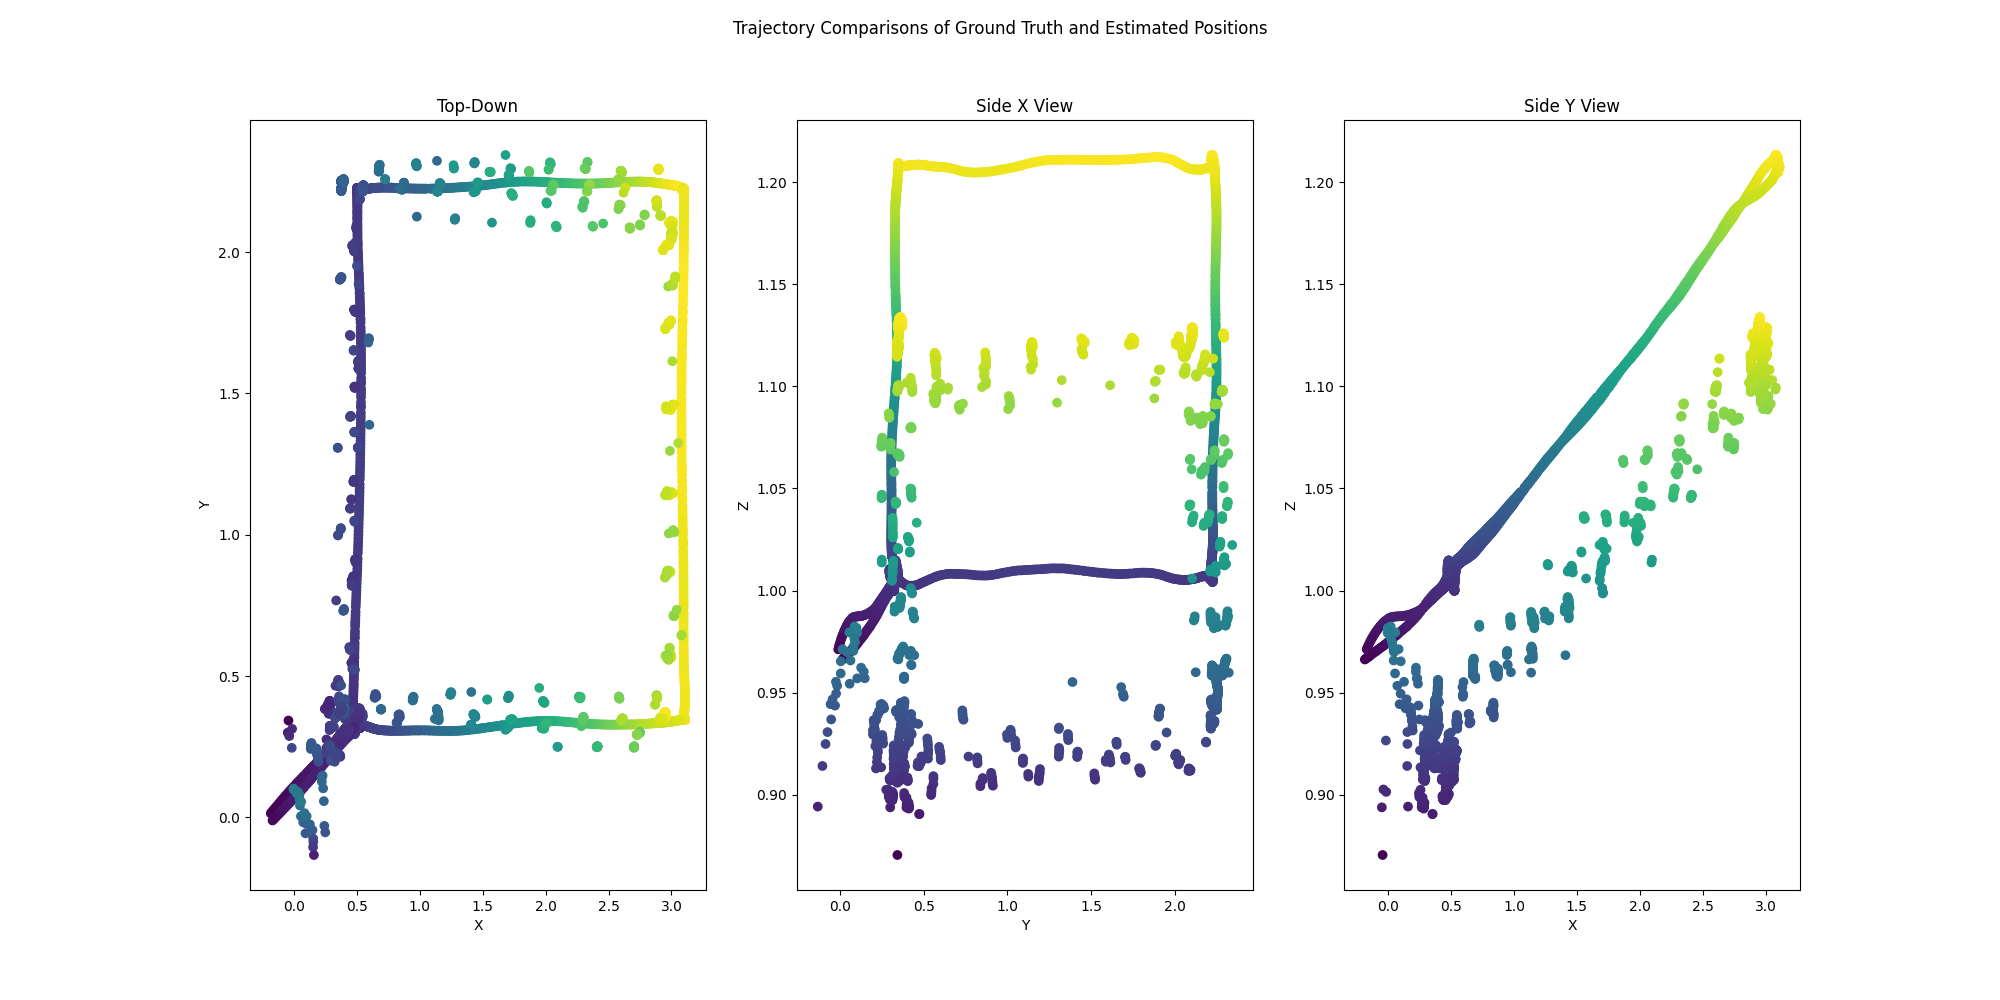
\includegraphics[width=0.8\textwidth]{./imgs/task1_2/studentdata5_trajectory_merged.png}
    \caption{Dataset 5 Trajectories}
\end{figure}

\begin{figure}[H]
    \centering
    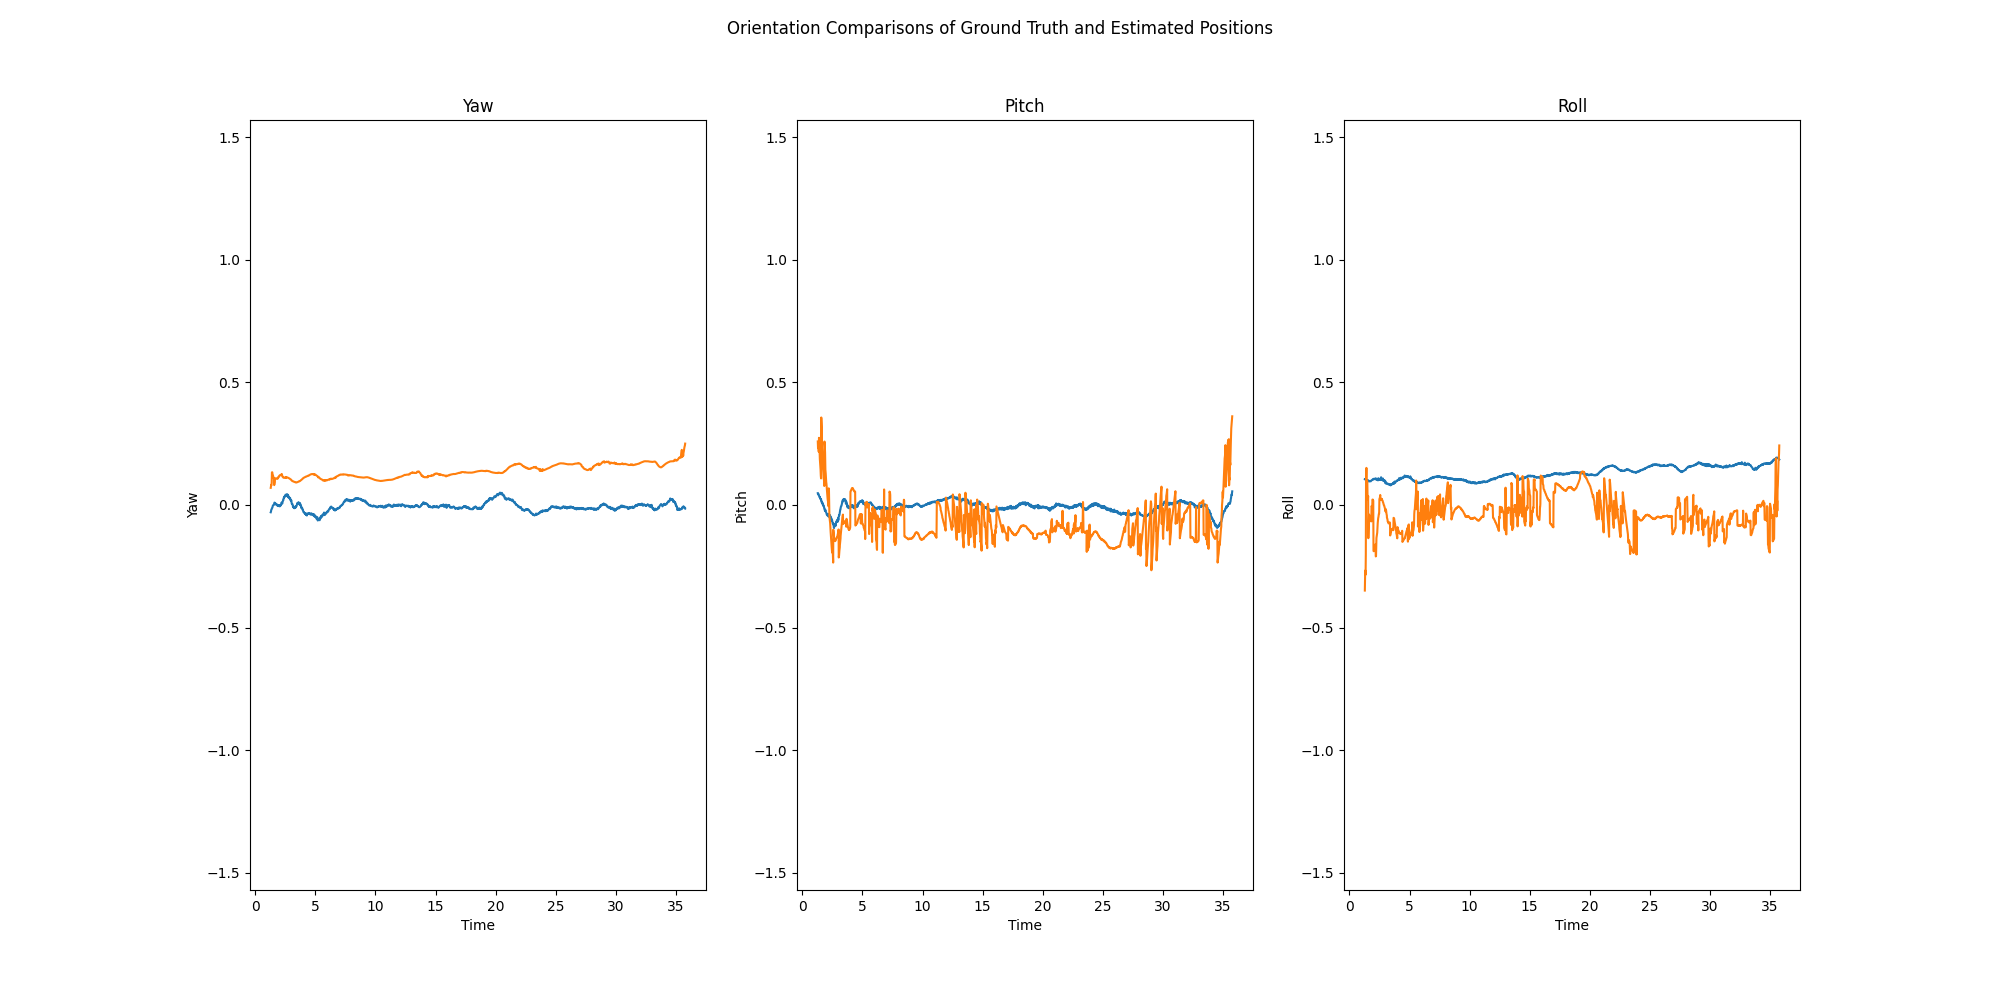
\includegraphics[width=0.8\textwidth]{./imgs/task1_2/studentdata5_orientation_merged.png}
    \caption{Dataset 5 Orientations}
\end{figure}

\subsection*{Dataset 6}

\begin{figure}[H]
    \centering
    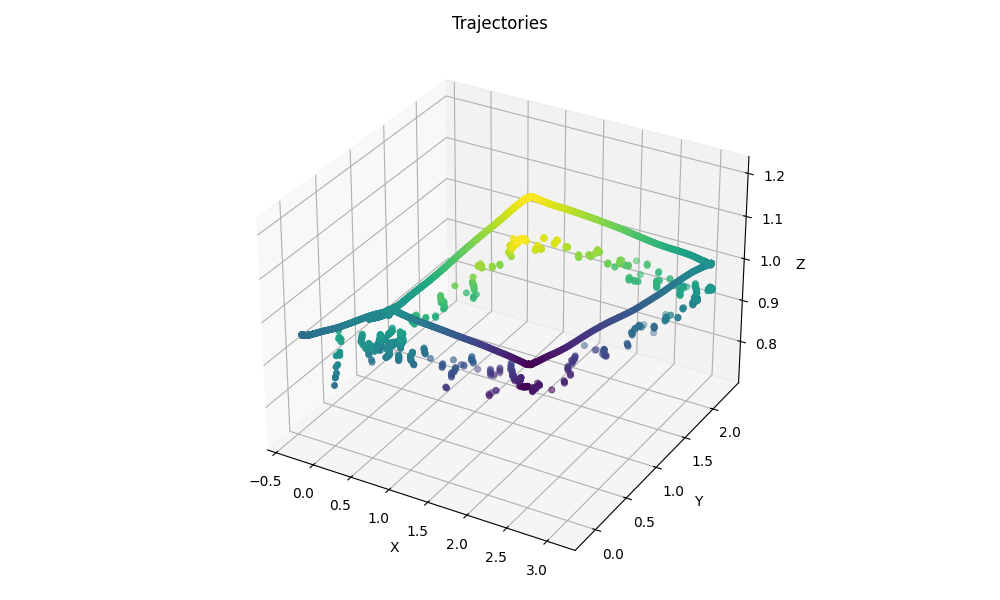
\includegraphics[width=0.8\textwidth]{./imgs/task1_2/studentdata6_isometric.png}
    \caption{Dataset 6 Isometric View}
\end{figure}

\begin{figure}[H]
    \centering
    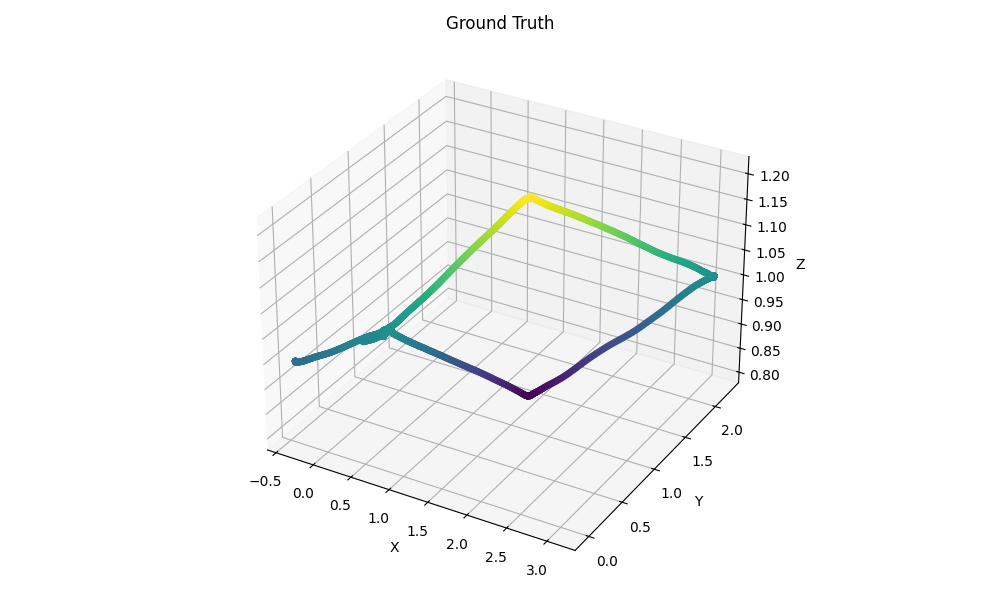
\includegraphics[width=0.8\textwidth]{./imgs/task1_2/studentdata6_ground_truth.png}
    \caption{Dataset 6 Ground Truth}
\end{figure}

\begin{figure}[H]
    \centering
    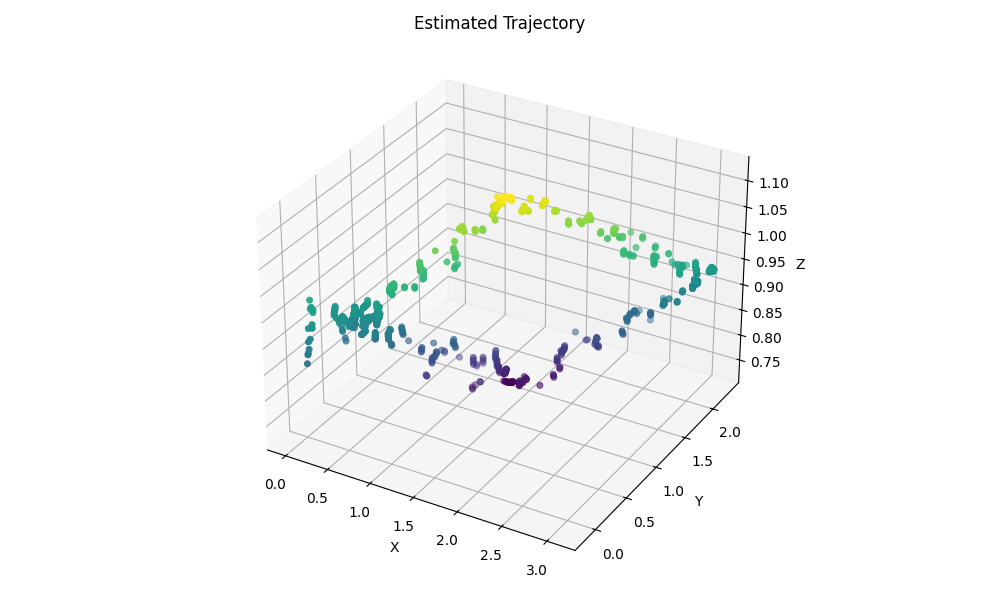
\includegraphics[width=0.8\textwidth]{./imgs/task1_2/studentdata6_estimated.png}
    \caption{Dataset 6 Estimated}
\end{figure}

\begin{figure}[H]
    \centering
    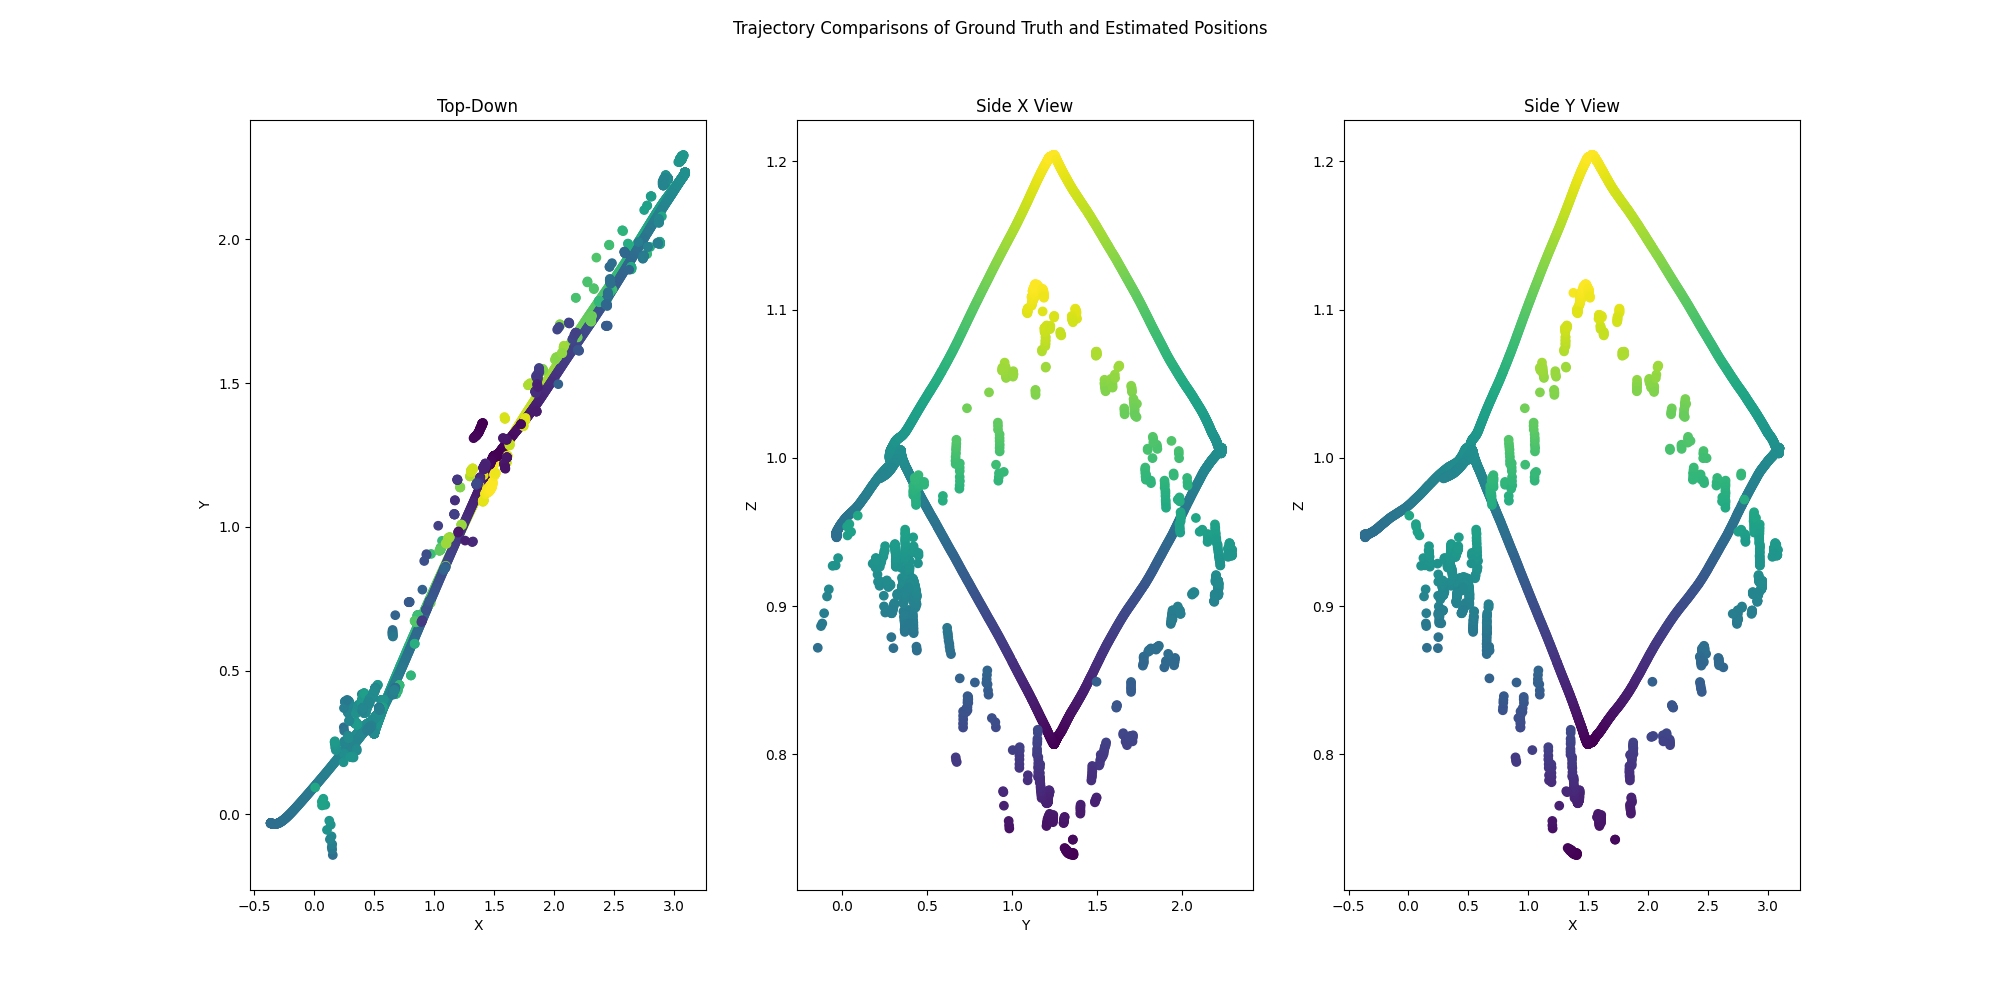
\includegraphics[width=0.8\textwidth]{./imgs/task1_2/studentdata6_trajectory_merged.png}
    \caption{Dataset 6 Trajectories}
\end{figure}

\begin{figure}[H]
    \centering
    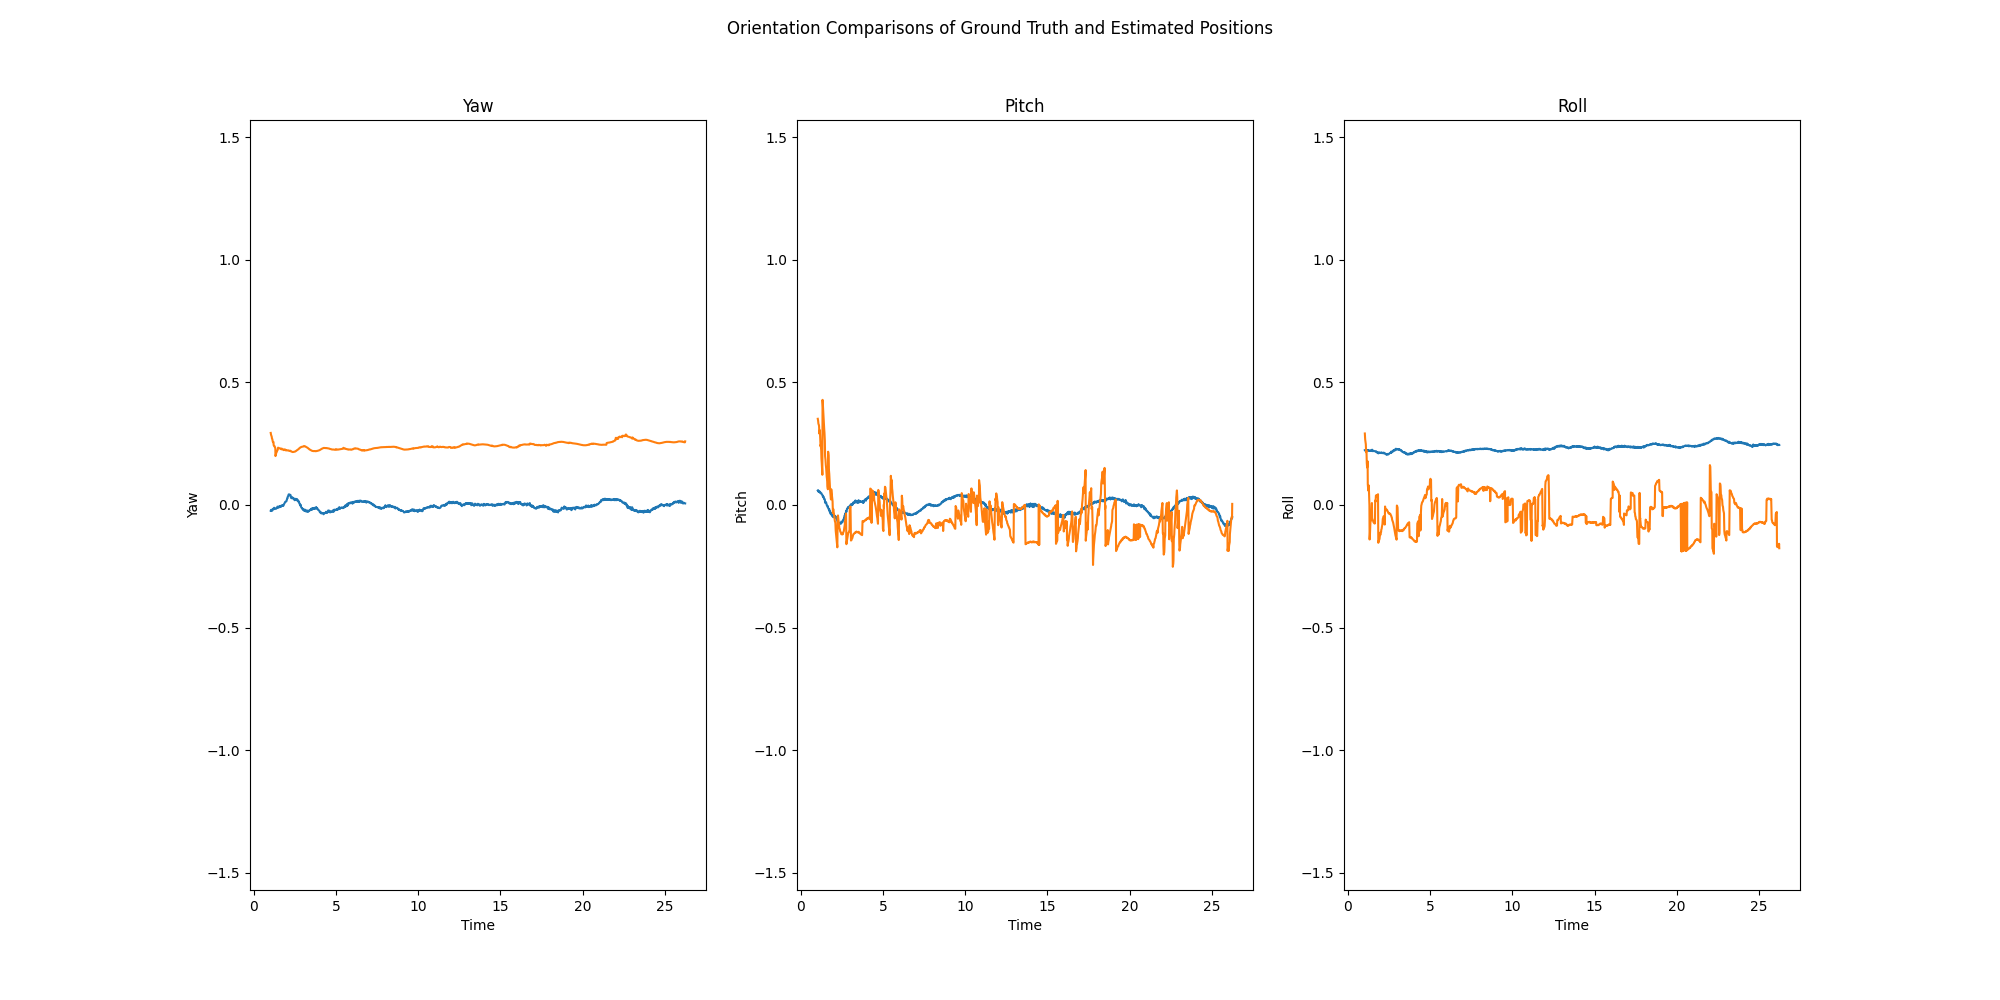
\includegraphics[width=0.8\textwidth]{./imgs/task1_2/studentdata6_orientation_merged.png}
    \caption{Dataset 6 Orientations}
\end{figure}

\subsection*{Dataset 7}

\begin{figure}[H]
    \centering
    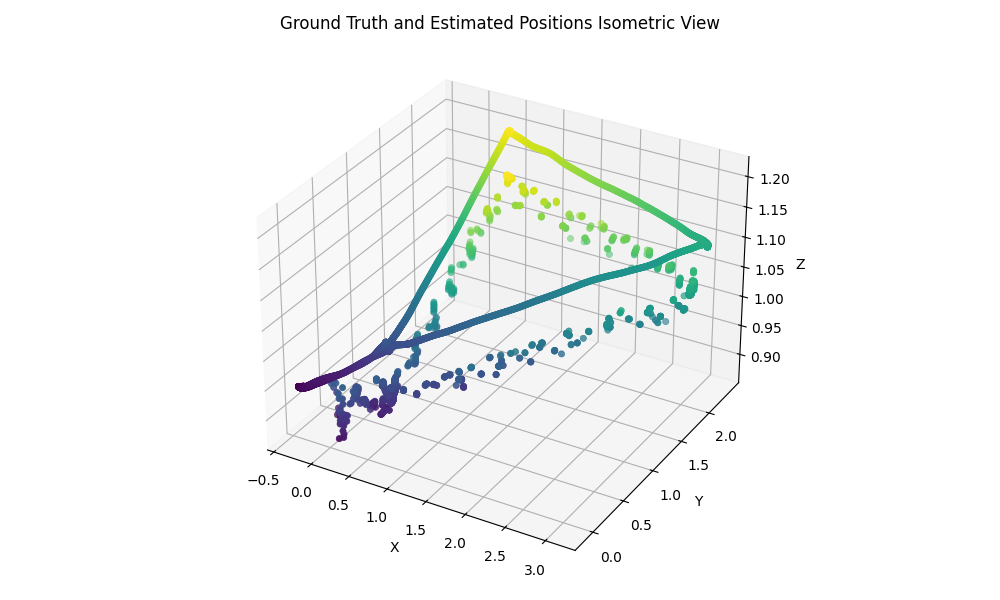
\includegraphics[width=0.8\textwidth]{./imgs/task1_2/studentdata7_isometric.png}
    \caption{Dataset 7 Isometric View}
\end{figure}

\begin{figure}[H]
    \centering
    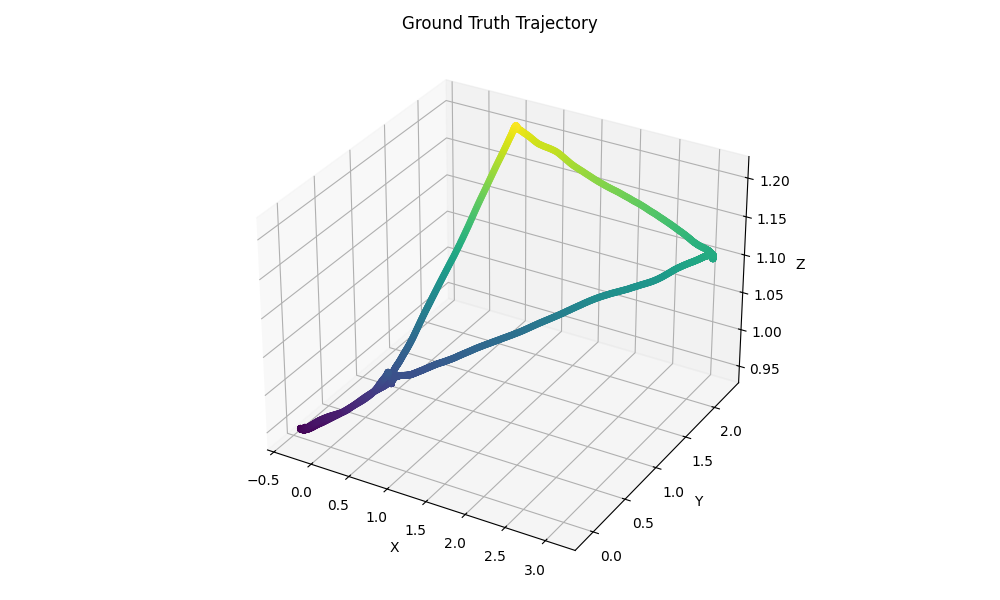
\includegraphics[width=0.8\textwidth]{./imgs/task1_2/studentdata7_ground_truth.png}
    \caption{Dataset 7 Ground Truth}
\end{figure}

\begin{figure}[H]
    \centering
    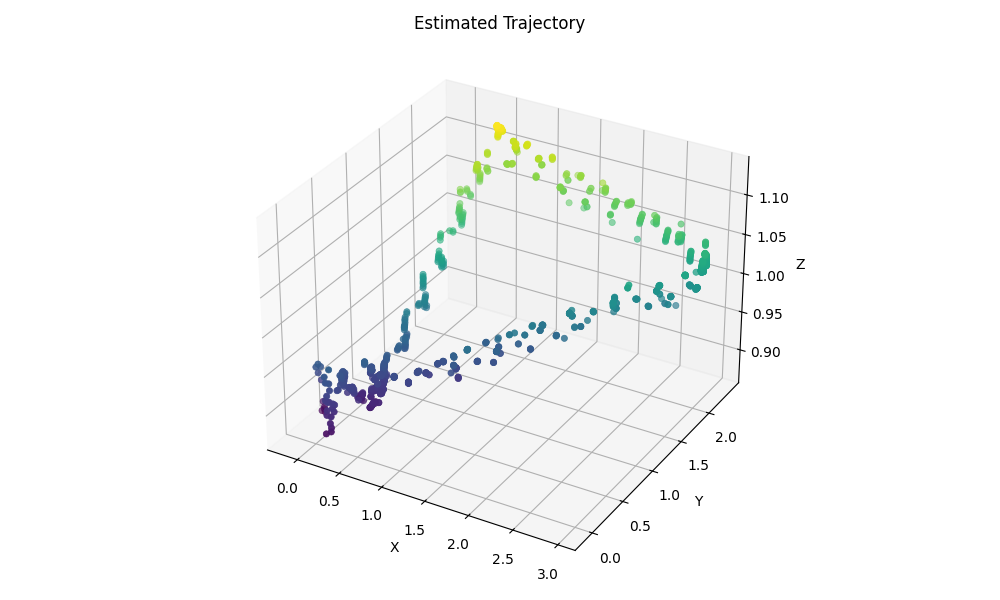
\includegraphics[width=0.8\textwidth]{./imgs/task1_2/studentdata7_estimated.png}
    \caption{Dataset 7 Estimated}
\end{figure}

\begin{figure}[H]
    \centering
    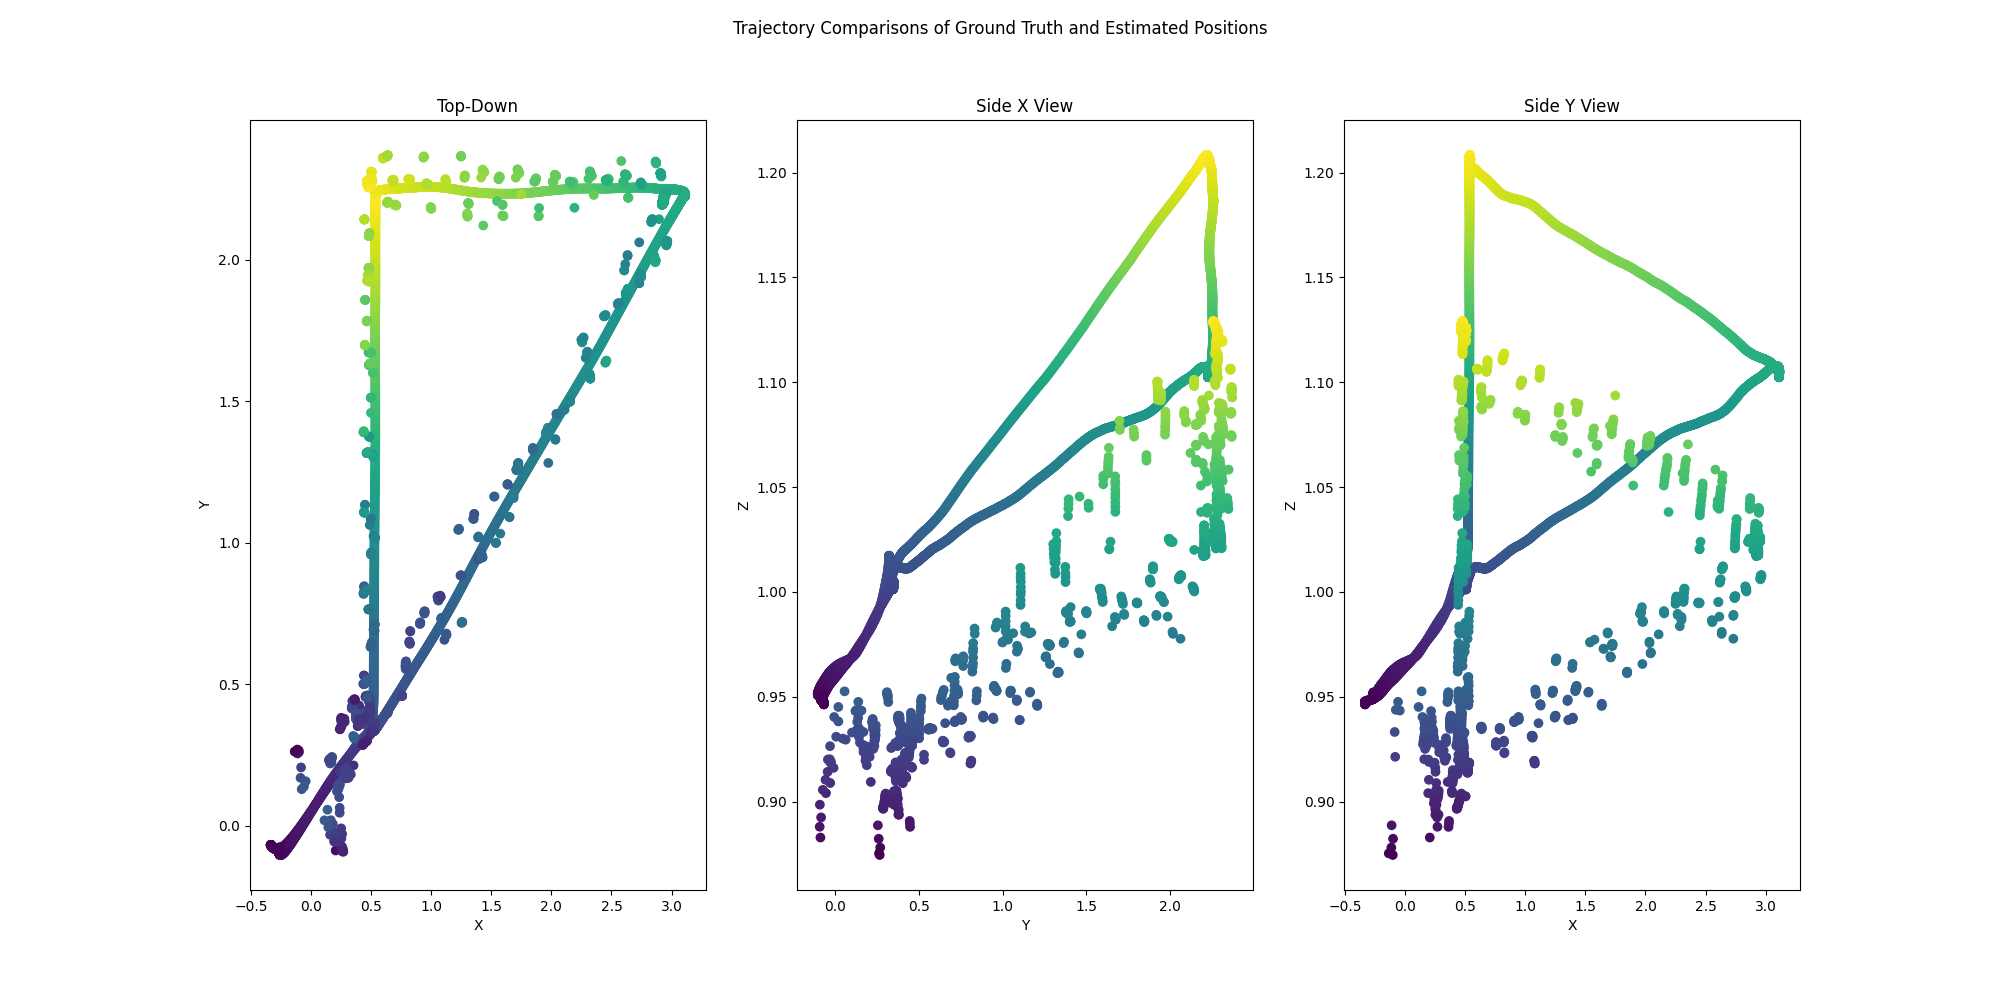
\includegraphics[width=0.8\textwidth]{./imgs/task1_2/studentdata7_trajectory_merged.png}
    \caption{Dataset 7 Trajectories}
\end{figure}

\begin{figure}[H]
    \centering
    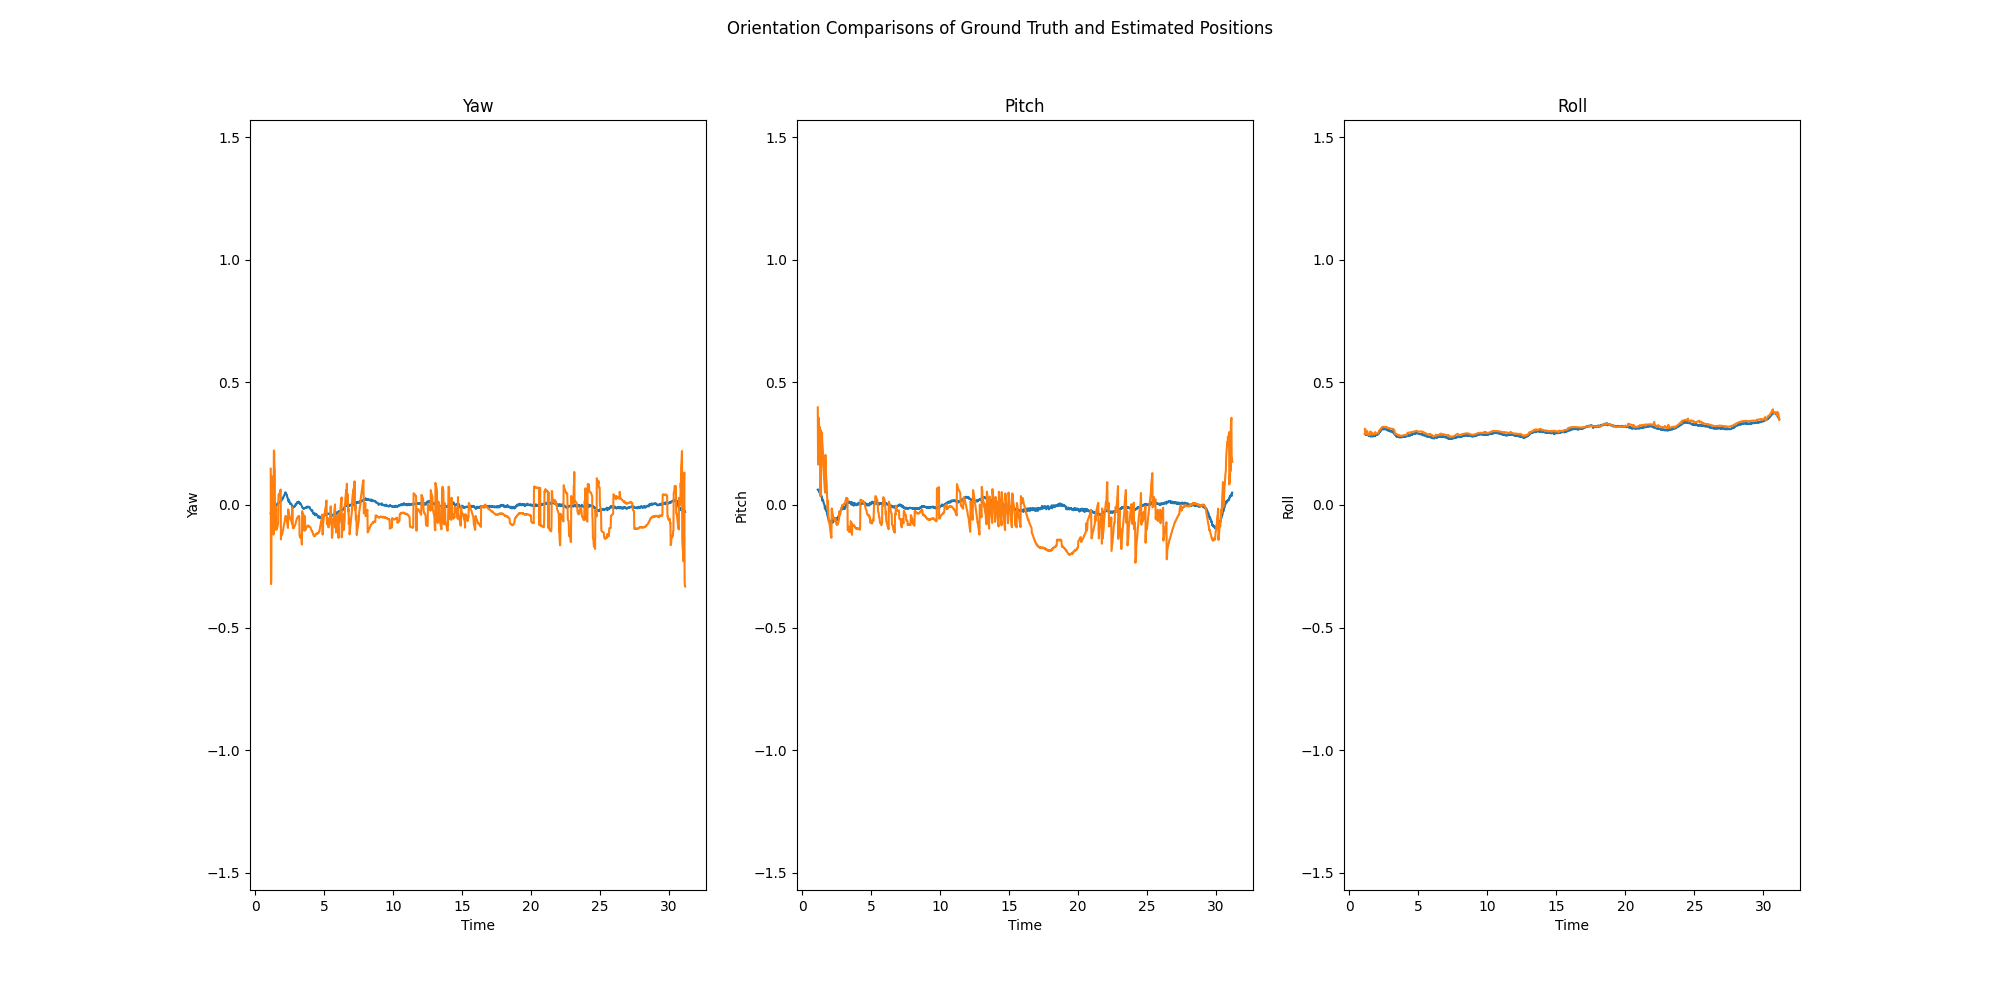
\includegraphics[width=0.8\textwidth]{./imgs/task1_2/studentdata7_orientation_merged.png}
    \caption{Dataset 7 Orientations}
\end{figure}


\section*{Task 3}

Task 3 asks us to calculate the covariance matrix for each dataset, and finally average them to create an experimentally derived covariance matrix for the our drone setup. To calculate this, we need to calculate $v_t$, which is the error of our estimated to ground truth states. Then we can solve for a given covariance matrix via:

\begin{equation}
    R = \frac{1}{N-1} \sum_{t=1}^n v_t v_t^T
\end{equation}

...where $R$ is our covariance matrix and $N$ is the number of estimated samples we're utilizing.

To solve this, the attached \textbf{task3.py} contains code that performs two key calculations; the first is \textit{interpolate\_ground\_truth}, which, given a set of ground truths and a given estimated position, linearly interpolates the surrounding set of ground truths to the same timestamp of the estimated position to find a more accurate point to compare against for our error. Ultimately, given an estimated position of timestamp $t_e$, we find the surrounding ground truth points at $t_a$ and $t_b$, where $t_a <= t_e <= t_b$. We then calculate the resulting interpolation $X_i$ via:

\begin{equation}
    X_i = (1 - \frac{t_e - t_a}{t_b - t_a})X_a + ()\frac{t_e - t_a}{t_b - t_a}) X_b
\end{equation}

The code for this is as follows:

\begin{python}
    def interpolate_ground_truth(gts: List[GroundTruth], estimation: Data) -> np.ndarray:
    # Interpolate the ground truth to the same times as the estimated
    # positions. Essentially, ground truths are recorded at a higher
    # cadence but not necessarily at the same time as the data point;
    # as such, we need to find the two times that surround our given
    # data point timestep and then find the resulting interpolation
    # between those, weighted based on time delta from each.
    #
    # Returns an numpy array (6,1) of the interpolated state vector

    # Get the current timestep from the estimation
    timestamp = estimation.timestamp

    # Find the first ground truth time that is past that timestamp
    a: GroundTruth = None
    b: GroundTruth = None
    for index, gt in enumerate(gts):
    # Skip the first ground truth
    if index == 0:
    continue
    if gt.timestamp > timestamp:
    a = gts[index - 1]
    b = gts[index]
    break
    if a is None or b is None:
    raise ValueError("No ground truth found for given timestamp")

    # Calculate our deltas to each timestamp. We will use this to form a
    # weight for each ground truth state vector for our averaging
    delta_a = timestamp - a.timestamp
    delta_b = b.timestamp - timestamp
    total_delta = b.timestamp - a.timestamp

    percentage_a = delta_a / total_delta
    percentage_b = delta_b / total_delta

    # Finally we create our new interpolated state vector by finding the
    # weighted average between a and b given our percentages as weights
    vector_a = np.array([a.x, a.y, a.z, a.roll, a.pitch, a.yaw]).reshape(6, 1)
    vector_b = np.array([b.x, b.y, b.z, b.roll, b.pitch, b.yaw]).reshape(6, 1)

    interpolated_state = (1 - percentage_a) * vector_a
    interpolated_state += (1 - percentage_b) * vector_b

    # Create a new ground truth object with the interpolated state vector
    return interpolated_state
\end{python}

We then have the \textit{estimate\_covariances} function, which, given our estimated data points and ground truths, will find the covariances for each estimated position, finally averaging them as we discussed above. Note that for some datasets we have estimated positions prior to the first ground truth recording; for this, we ignore each of the estimates in our calculations.

The code for \textit{estimate\_covariances} is as follows:

\begin{python}
    def estimate_covariances(
    gt: List[GroundTruth],
    positions: List[np.ndarray],
    orientations: List[np.ndarray],
    data: List[Data],
    ) -> np.ndarray:
    covariances: List[np.ndarray] = []
    count = 0

    # covariances = np.zeros((6, 6))
    for index, position in enumerate(positions):
    # If the drone positions predates the first timestamp of our
    # ground truth, we can't properly interpolate or really
    # calculate a covariance off of it, so we ignore it
    if data[index].timestamp < gt[0].timestamp:
    continue

    count += 1

    # Interpolate the ground truth to the same time as the
    # estimated position
    interpolated = interpolate_ground_truth(gt, data[index])

    # Calculate the difference between the interpolated ground
    # truth and the estimated position
    position_vector = np.array(
    [
            position[0],
            position[1],
            position[2],
            orientations[index][0],
            orientations[index][1],
            orientations[index][2],
        ]
    ).reshape(6, 1)
    error = interpolated - position_vector

    # Calculate the covariance matrix
    covariance = np.dot(error, error.T)
    # covariances += covariance
    covariances.append(covariance)

    # Now that we have all of the 6x6 covariance matricies, we need
    # to find the average of them all
    average_covariance = (1 / (len(covariances) - 1)) * np.sum(covariances, axis=0)

    return average_covariance
\end{python}

The results for each of these are as follows:

\noindent\textbf{Dataset 0}

\begin{equation}
    \begin{bmatrix}
        0.01124642  & -0.00167306 & -0.00189018 & -0.00242393 & -0.00395184 & 0.00753254  \\
        -0.00167306 & 0.00544109  & 0.0002523   & -0.00356955 & 0.00328967  & -0.00228468 \\
        -0.00189018 & 0.0002523   & 0.00119225  & 0.00075236  & 0.0027241   & -0.00231984 \\
        -0.00242393 & -0.00356955 & 0.00075236  & 0.00573034  & 0.00215346  & -0.00260745 \\
        -0.00395184 & 0.00328967  & 0.0027241   & 0.00215346  & 0.01472657  & -0.00911272 \\
        0.00753254  & -0.00228468 & -0.00231984 & -0.00260745 & -0.00911272 & 0.00856904  \\
    \end{bmatrix}
\end{equation}

\noindent\textbf{Dataset 1}
\begin{equation}
    \begin{bmatrix}
        4.01277933e-03 & 1.18288647e-03  & -2.00353030e-03 & -5.74159527e-04 & 2.58453957e-03  & 3.31938031e-04  \\
        1.18288647e-03 & 5.43967539e-03  & -4.66980820e-03 & -3.87141261e-03 & 5.64105295e-04  & 5.92553237e-04  \\
        2.00353030e-03 & -4.66980820e-03 & 1.24291009e-02  & 2.44736338e-03  & -2.65707665e-04 & -1.24055364e-03 \\
        5.74159527e-04 & -3.87141261e-03 & 2.44736338e-03  & 3.53193690e-03  & -3.22706410e-04 & -3.36813351e-04 \\
        2.58453957e-03 & 5.64105295e-04  & -2.65707665e-04 & -3.22706410e-04 & 2.63705969e-03  & 4.27377172e-05  \\
        3.31938031e-04 & 5.92553237e-04  & -1.24055364e-03 & -3.36813351e-04 & 4.27377172e-05  & 1.89300698e-04  \\
    \end{bmatrix}
\end{equation}

\noindent\textbf{Dataset 2}

\begin{equation}
    \begin{bmatrix}
        4.86409531e-03  & -2.94125078e-04 & 2.32462827e-03  & 1.87162183e-03  & 3.41062843e-03  & -8.91656484e-05 \\
        -2.94125078e-04 & 3.75937724e-03  & 3.06819200e-04  & -1.96590128e-03 & 1.44735836e-03  & -1.99711265e-04 \\
        2.32462827e-03  & 3.06819200e-04  & 1.58949347e-02  & 4.23769157e-03  & 3.55140819e-03  & -1.94017055e-03 \\
        1.87162183e-03  & -1.96590128e-03 & 4.23769157e-03  & 3.41537425e-03  & 9.04672800e-04  & -4.90091508e-04 \\
        3.41062843e-03  & 1.44735836e-03  & 3.55140819e-03  & 9.04672800e-04  & 3.91137920e-03  & -3.76095525e-04 \\
        -8.91656484e-05 & -1.99711265e-04 & -1.94017055e-03 & -4.90091508e-04 & -3.76095525e-04 & 3.21519940e-04  \\
    \end{bmatrix}
\end{equation}

\noindent\textbf{Dataset 3}

\begin{equation}
    \begin{bmatrix}
        3.52547293e-03 & -4.72620065e-04 & 3.07029719e-03  & 6.22102878e-05  & 3.67552366e-03  & -9.46301282e-05 \\
        4.72620065e-04 & 3.88425041e-03  & -1.96856899e-03 & -3.17453865e-03 & 9.18529526e-05  & 1.74223365e-04  \\
        3.07029719e-03 & -1.96856899e-03 & 9.63698086e-03  & 1.04535253e-03  & 3.89692176e-03  & -7.68074907e-04 \\
        6.22102878e-05 & -3.17453865e-03 & 1.04535253e-03  & 3.43191599e-03  & -3.66936788e-04 & -1.29199561e-04 \\
        3.67552366e-03 & 9.18529526e-05  & 3.89692176e-03  & -3.66936788e-04 & 4.64044464e-03  & -1.70354010e-04 \\
        9.46301282e-05 & 1.74223365e-04  & -7.68074907e-04 & -1.29199561e-04 & -1.70354010e-04 & 1.34914826e-04  \\
    \end{bmatrix}
\end{equation}

\noindent\textbf{Dataset 4}

\begin{equation}
    \begin{bmatrix}
        5.80720160e-03  & 1.14209446e-03  & -3.32687103e-03 & -4.51481879e-03 & -2.22035532e-03 & 5.58421955e-04  \\
        1.14209446e-03  & 3.76246524e-03  & -1.65576059e-03 & -1.17842357e-03 & -2.34043302e-03 & 8.15228628e-05  \\
        -3.32687103e-03 & -1.65576059e-03 & 1.20429769e-02  & -2.09502222e-03 & 3.12967094e-03  & -5.49304255e-04 \\
        -4.51481879e-03 & -1.17842357e-03 & -2.09502222e-03 & 9.28640486e-03  & 1.87405911e-03  & -5.15425799e-04 \\
        -2.22035532e-03 & -2.34043302e-03 & 3.12967094e-03  & 1.87405911e-03  & 5.40791117e-03  & -2.87277973e-04 \\
        5.58421955e-04  & 8.15228628e-05  & -5.49304255e-04 & -5.15425799e-04 & -2.87277973e-04 & 1.84442372e-04  \\
    \end{bmatrix}
\end{equation}

\noindent\textbf{Dataset 5}

\begin{equation}
    \begin{bmatrix}
        1.18828159e-02  & -1.57135877e-04 & 6.84362005e-03  & 2.75507433e-03  & 1.11343543e-02  & -5.18876334e-04 \\
        -1.57135877e-04 & 5.11853661e-03  & -7.00718409e-04 & -4.64546311e-03 & 1.01445288e-03  & 1.04231491e-04  \\
        6.84362005e-03  & -7.00718409e-04 & 7.22308207e-03  & 2.18075250e-03  & 6.07548527e-03  & -6.58825680e-04 \\
        2.75507433e-03  & -4.64546311e-03 & 2.18075250e-03  & 4.87070199e-03  & 1.51707136e-03  & -1.91024090e-04 \\
        1.11343543e-02  & 1.01445288e-03  & 6.07548527e-03  & 1.51707136e-03  & 1.08072792e-02  & -4.44675170e-04 \\
        -5.18876334e-04 & 1.04231491e-04  & -6.58825680e-04 & -1.91024090e-04 & -4.44675170e-04 & 8.23956082e-05  \\
    \end{bmatrix}
\end{equation}

\noindent\textbf{Dataset 6}

\begin{equation}
    \begin{bmatrix}
        7.56080877e-03  & 2.58498816e-04  & 4.26804240e-03  & 2.78682407e-03  & 7.68447496e-03  & -4.19928996e-04 \\
        2.58498816e-04  & 5.38572490e-03  & -4.66333273e-04 & -5.30269266e-03 & 2.11255935e-03  & 3.10509562e-05  \\
        4.26804240e-03  & -4.66333273e-04 & 6.33646109e-03  & 2.23178635e-03  & 3.96139946e-03  & -7.22476457e-04 \\
        2.78682407e-03  & -5.30269266e-03 & 2.23178635e-03  & 6.59630424e-03  & 1.00365272e-03  & -1.90238025e-04 \\
        7.68447496e-03  & 2.11255935e-03  & 3.96139946e-03  & 1.00365272e-03  & 8.61378814e-03  & -3.98425477e-04 \\
        -4.19928996e-04 & 3.10509562e-05  & -7.22476457e-04 & -1.90238025e-04 & -3.98425477e-04 & 1.07436905e-04  \\
    \end{bmatrix}
\end{equation}

\noindent\textbf{Dataset 7}

\begin{equation}
    \begin{bmatrix}
        0.00787652  & 0.0002269   & 0.00462655  & 0.00362929  & 0.00697831  & -0.00029106 \\
        0.0002269   & 0.00483996  & -0.00177252 & -0.00401243 & 0.0024168   & 0.00014734  \\
        0.00462655  & -0.00177252 & 0.00731506  & 0.00361734  & 0.00315442  & -0.00074367 \\
        0.00362929  & -0.00401243 & 0.00361734  & 0.00530187  & 0.00134563  & -0.00023165 \\
        0.00697831  & 0.0024168   & 0.00315442  & 0.00134563  & 0.0072551   & -0.00016959 \\
        -0.00029106 & 0.00014734  & -0.00074367 & -0.00023165 & -0.00016959 & 0.00010396  \\
    \end{bmatrix}
\end{equation}

...and finally, when we average them together, we get a final covariance matrix of:

\begin{equation}
    \begin{bmatrix}
        7.09701409e-03 & 2.66809900e-05  & 1.73906943e-03  & 4.49014777e-04  & 3.66195490e-03  & 8.76154421e-04  \\
        2.66809900e-05 & 4.70388499e-03  & -1.33432420e-03 & -3.46505064e-03 & 1.07454548e-03  & -1.69184839e-04 \\
        1.73906943e-03 & -1.33432420e-03 & 9.00885499e-03  & 1.80220246e-03  & 3.27846190e-03  & -1.11786368e-03 \\
        4.49014777e-04 & -3.46505064e-03 & 1.80220246e-03  & 5.27060654e-03  & 1.01361187e-03  & -5.86487142e-04 \\
        3.66195490e-03 & 1.07454548e-03  & 3.27846190e-03  & 1.01361187e-03  & 7.24994152e-03  & -1.36454993e-03 \\
        8.76154421e-04 & -1.69184839e-04 & -1.11786368e-03 & -5.86487142e-04 & -1.36454993e-03 & 1.21162646e-03  \\
    \end{bmatrix}
\end{equation}

\section*{Task 4}

Coming soon...

\end{document}